\chapter{Vuelo Circular}

El último caso de vuelo a analizar es el del vuelo circular, un vuelo a nivel siguiendo una trayectoria curvilínea de radio constante. Se ha escogido esta trayectoria por ser una que puede ser empleada en misiones de vigilancia de un terreno concreto. 
Se analizará la influencia de la velocidad y el radio de giro de la trayectoria en el vuelo de la aeronave para después comprobar el efecto de modificaciones sobre los parámetros de diseño de la misma. El caso inicial es de un vuelo a 1000 m de altitud con un radio de giro de 300 m. 

\begin{figure}
	\centering
	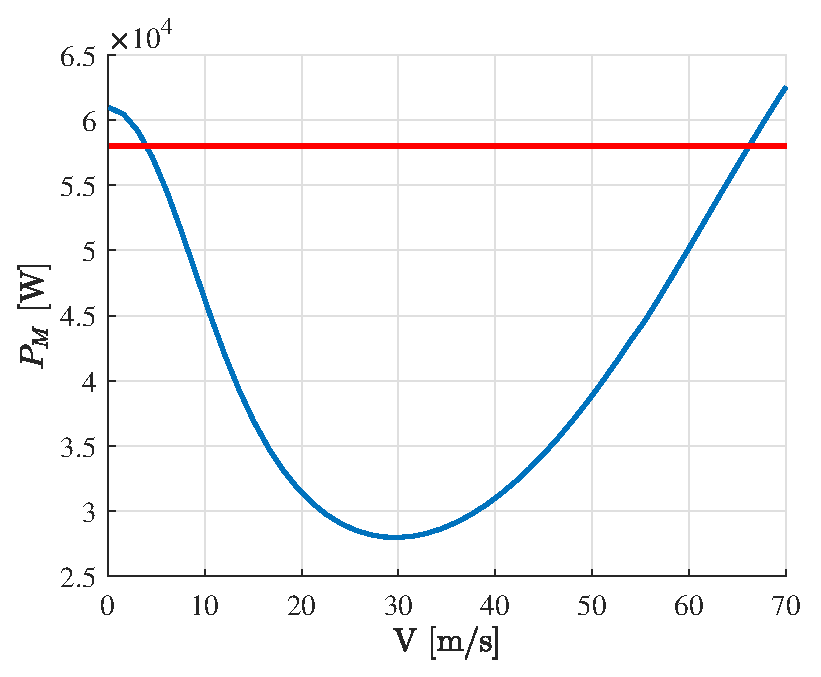
\includegraphics[width=90mm]{graficos/PMVC}
	\caption{Consumo de Potencia de la aeronave en función de la velocidad de vuelo a una altitud de 1000 m para vuelo circular de radio 300 m y limitación por potencia máxima continua disponible.}
	\label{PMVC}
\end{figure}

Como se puede observar en la gráfica \ref{PMVC}, el consumo mínimo de potencia se ha desplazado, dándose para una velocidad de vuelo de 30.0275 m/s, siendo dicha potencia de 27.99 kW. En lo referente a la velocidad máxima, esta se sitúa en 66.2 m/s, un poco por debajo del caso para vuelo horizontal.

\begin{figure}
	\centering
	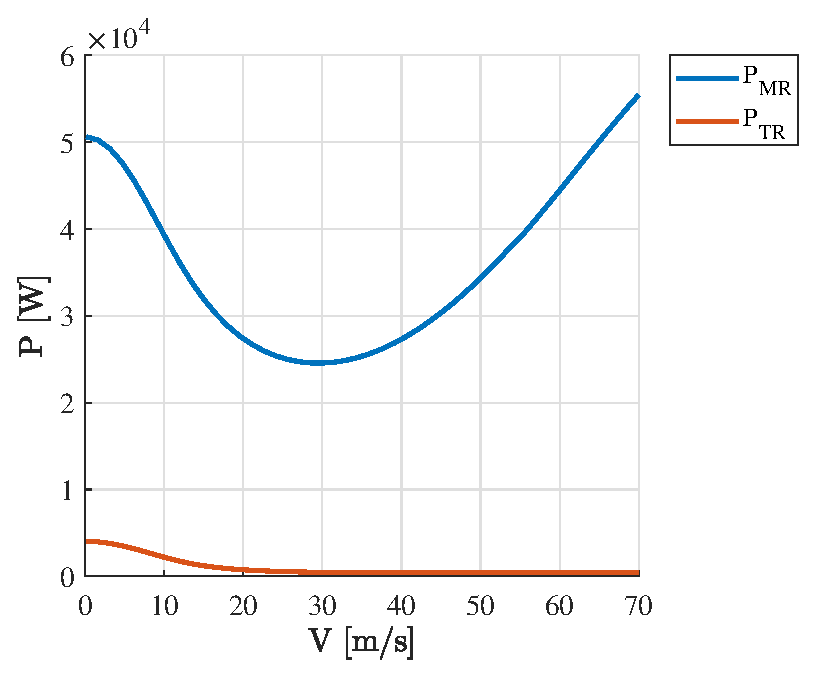
\includegraphics[width=90mm]{graficos/PVC}
	\caption{Consumo de Potencia de los rotores principal y antipar en función de la velocidad de vuelo a una altitud de 1000 m para vuelo circular de radio 300 m.}
	\label{PVC}
\end{figure}
\begin{figure}
	\centering
	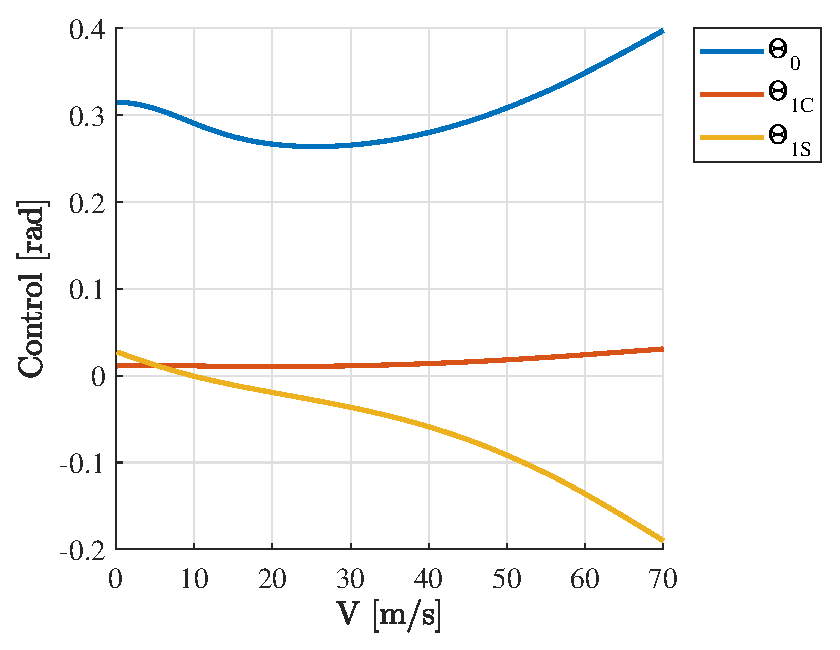
\includegraphics[width=90mm]{graficos/ControlVC}
	\caption{Ángulos de control de la aeronave en función de la velocidad de vuelo a una altitud de 1000 m para vuelo circular de radio 300 m.}
	\label{ControlVC}
\end{figure}
\begin{figure}
	\centering
	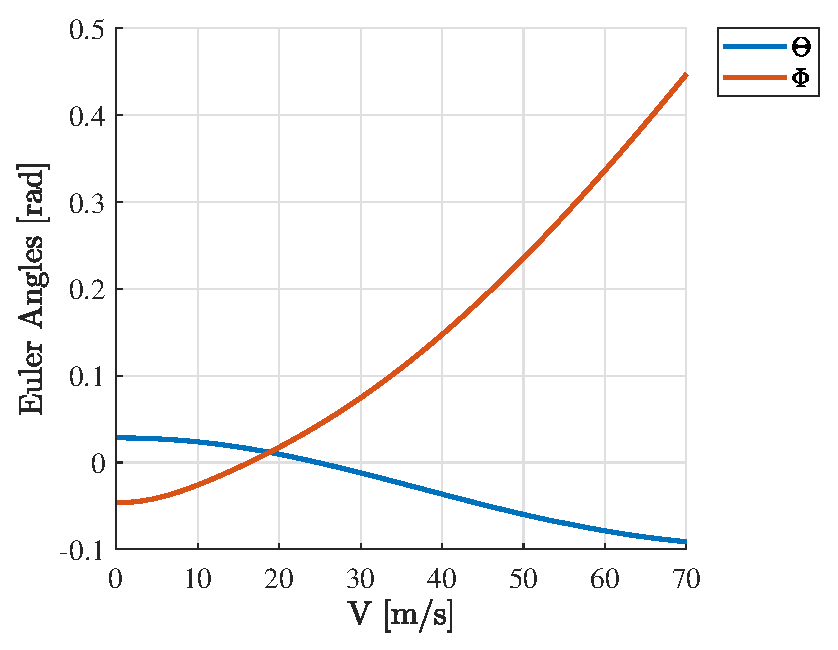
\includegraphics[width=90mm]{graficos/EulerVC}
	\caption{Ángulos de Euler de la aeronave en función de la velocidad de vuelo a una altitud de 1000 m para vuelo circular de radio 300 m.}
	\label{EulerVC}
\end{figure}

Respecto al resto de parámetros, solo resulta llamativo el ángulo de balanceo que se encuentra en la gráfica \ref{EulerVC}. Dicho ángulo crece con la velocidad debido a la necesidad de mantener una trayectoria circular cuyo radio es constante.
El resto de resultados no resultan extraños, por lo que nos sirven para comprobar que se han hecho los cálculos correctamente.


\section{Autonomía de Vuelo}

En este tipo de vuelo la autonomía vuelve a cobrar relevancia ya que durante una misión de vigilancia esta podría ser la trayectoria que el vehículo mantuviese durante largos períodos de tiempo. Resulta interesante, por tanto, conocer cuanto tiempo puede estar volando antes de tener que sustituirlo.

Los cálculos de para la autonomía ya se expusieron en el capítulo 4, por lo que se omitirán, reflejando únicamente los resultados en la gráfica \ref{autonomiaVC} y la tabla \ref{auttablaVC}.

\begin{figure}
	\centering
	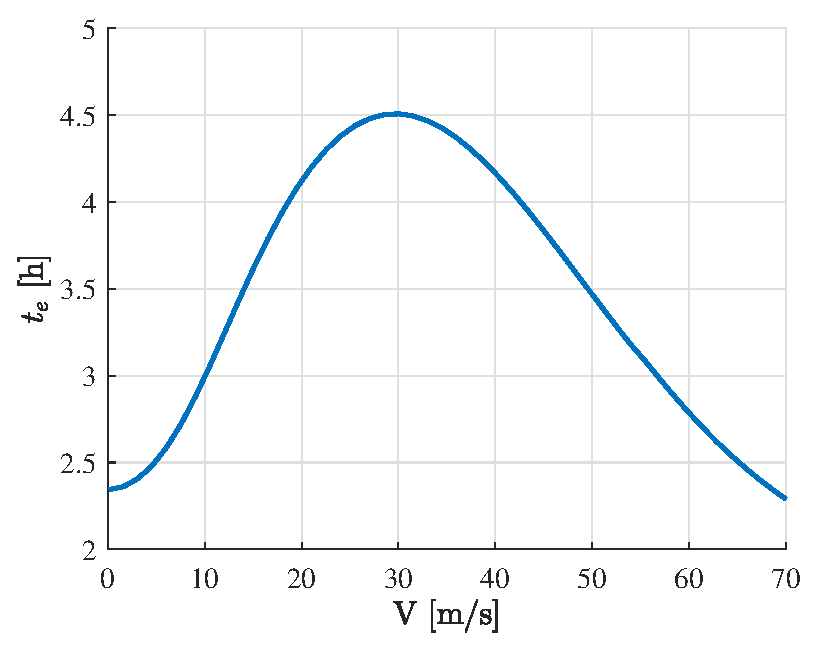
\includegraphics[width=90mm]{graficos/teVC}
	\caption{Autonomía de la aeronave en función de la velocidad de vuelo a una altitud de 100 m para vuelo circular de radio 300 m.}
	\label{autonomiaVC}
\end{figure}

\begin{table}[htbp]
	\centering
	\begin{tabular}{|>{\columncolor{Gray}}c|c|}
		\hline
		\cellcolor{Gray2}Variable & \cellcolor{Gray2}Valor \\ \hline \hline
		\cellcolor{Gray}Potencia para máxima autonomía ($P_{min,t_{e,max}}$)  & 27.99 kW \\ \hline
		\cellcolor{Gray}Velocidad en régimen de máxima autonomía ($V$) & 30.0275 m/s \\ \hline
		\cellcolor{Gray}Consumo específico en régimen de máxima autonomía ($c_{e,t_{e,max}}$) & 8.9234$\cdot$10$^-08$ kg/W$\cdot$s \\ \hline
		\cellcolor{Gray}Máxima autonomía ($t_{e,max}$) & 4.5043 h \\ \hline
	\end{tabular}%
	\caption{Parámetros relativos al cálculo de la máxima autonomía y su valor para un vuelo circular de radio 300 m a una altitud de 1000 m.}
	\label{auttablaVC}
\end{table}%

Como se puede ver, la autonomía máxima es de 4.5043 horas. Comparado con el resultado obtenido para vuelo horizontal a nivel del mar, 4.5887 horas, por lo que la disminución de la autonomía debida al cambio de condiciones no resulta muy perjudicial.

\section{Análisis de Varios Tipos de Misiones}

En este apartado se expondrán análisis de diversas misiones que interesan que sea capaz de realizar la aeronave, de manera que se obtengan sus actuaciones para las mismas.

\subsection*{Vuelos con Trayectorias de Diferentes Radios}

Otra condición de vuelo interesante es el radio de la trayectoria circular. Las misiones de vigilancia pueden requerir cubrir terrenos mas o menos grandes, con lo que conviene conocer el efecto de la trayectoria en las actuaciones del vehículo. Cabe destacar que se omitirá el análisis a bajas velocidades, ya que en estas condiciones los resultados no dependen igual del radio de la trayectoria.

\begin{figure}
	\centering
	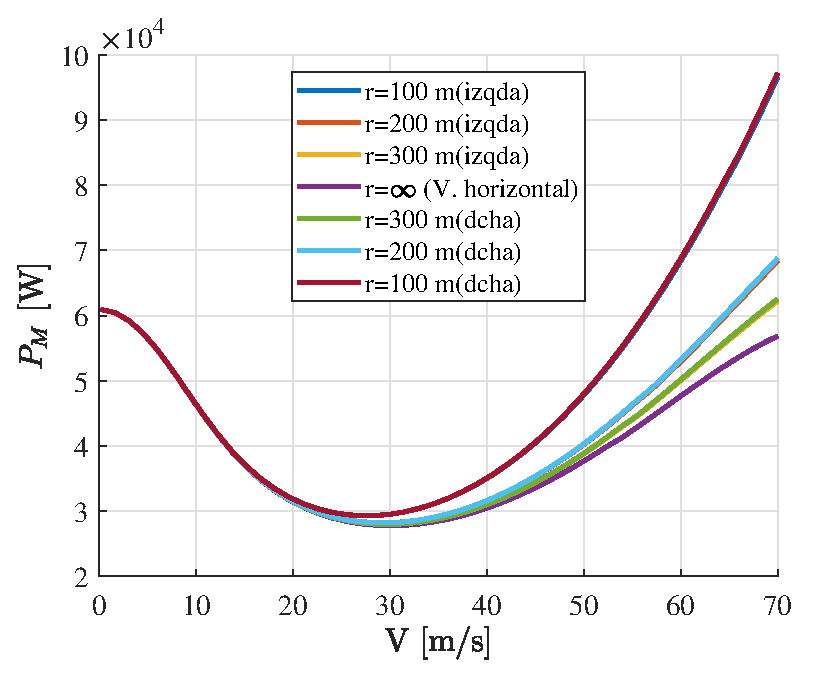
\includegraphics[width=90mm]{graficos/PMVCcs}
	\caption{Consumo de Potencia de la aeronave en función de la velocidad de vuelo a una altitud de 1000 m para vuelo circular de diferentes radios y limitación por potencia máxima continua disponible.}
	\label{PMVCcs}
\end{figure}

En la gráfica de potencias consumidas \ref{PMVCcs} se puede observar que la reducción del radio de giro conlleva un aumento exponencial de la potencia necesaria para llevar a cabo el vuelo independientemente de si el giro es hacia la derecha o la izquierda, lo que implica que para radios de giro de 100 m, las velocidades máximas de vuelo se ven limitadas a valores alrededor de 55.4 m/s (55.31 m/s para el giro a derechas y 55.44 m/s para el giro a izquierdas). A simple vista puede parecer que el sentido de giro es indiferente, pero los consumos de potencia resultan ligeramente mayores para giros a derechas que a izquierdas.

\begin{figure}
	\centering
	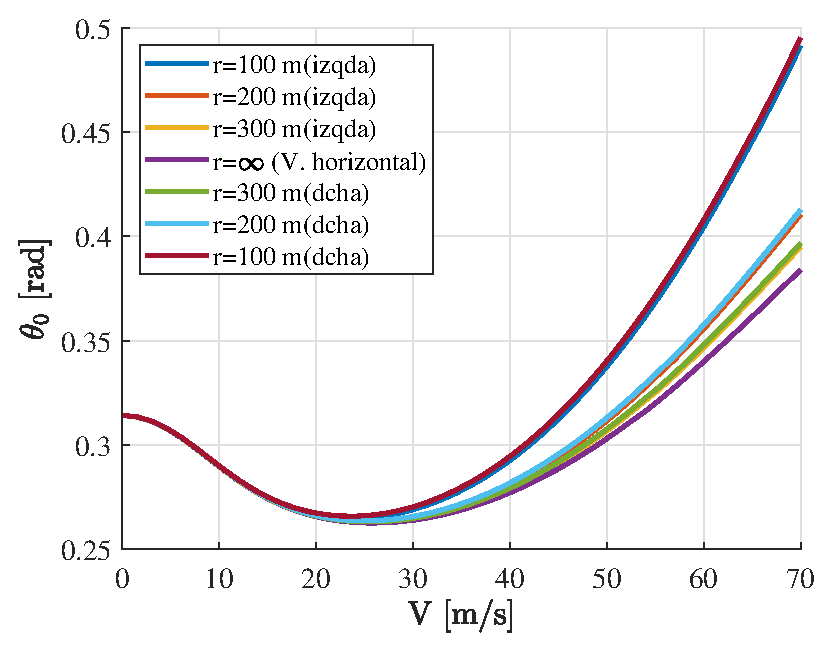
\includegraphics[width=90mm]{graficos/theta0VCcs}
	\caption{Ángulo de paso colectivo del rotor principal en función de la velocidad de vuelo a una altitud de 1000 m para vuelo circular de diferentes radios.}
	\label{theta0VCcs}
\end{figure}
\begin{figure}
	\centering
	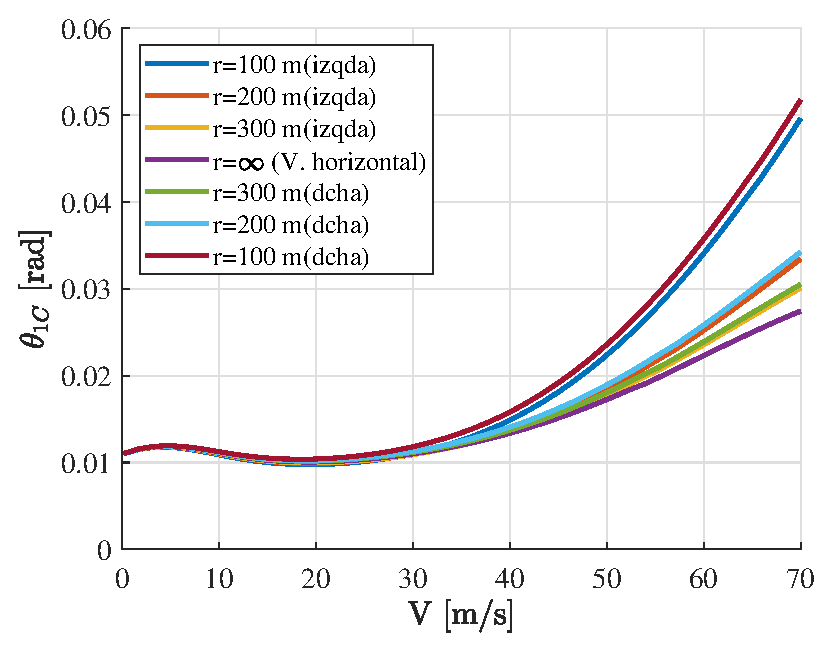
\includegraphics[width=90mm]{graficos/theta1CVCcs}
	\caption{Ángulo de paso cíclico longitudinal del rotor principal en función de la velocidad de vuelo a una altitud de 1000 m para vuelo circular de diferentes radios.}
	\label{theta1CVCcs}
\end{figure}
\begin{figure}
	\centering
	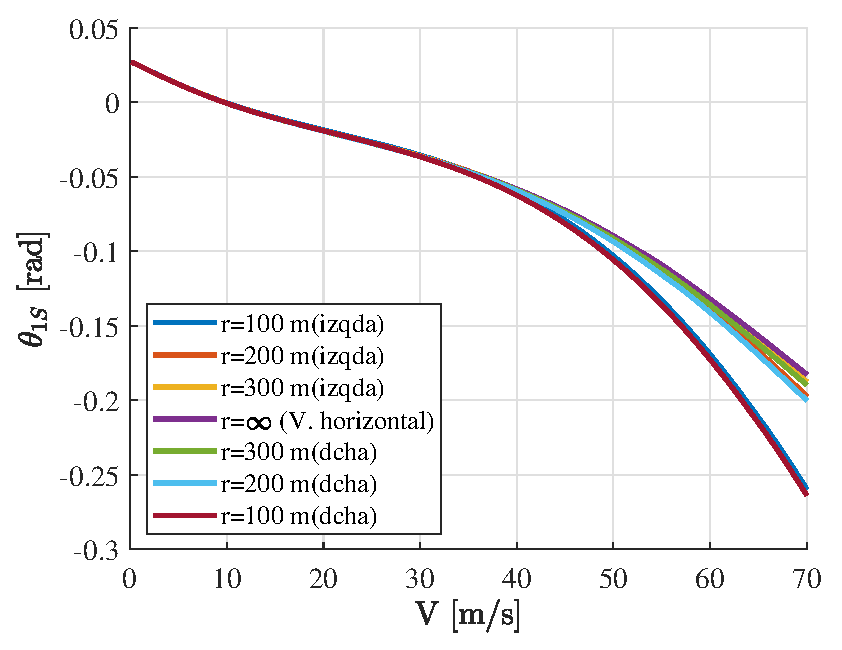
\includegraphics[width=90mm]{graficos/theta1SVCcs}
	\caption{Ángulo de paso cíclico lateral del rotor principal en función de la velocidad de vuelo a una altitud de 1000 m para vuelo circular de diferentes radios.}
	\label{theta1SVCcs}
\end{figure}

Los resultados de los ángulos de control del rotor principal se recogen en las gráficas \ref{theta0VCcs}, \ref{theta1CVCcs} y \ref{theta1SVCcs}. En ellas la evolución es similar al caso de la potencia, los valores absolutos de los ángulos se incrementan según reduce el ángulo de giro, y lo hacen de forma exponencial. De nuevo los datos parecen ir en parejas, pero las diferencias entre los giros a derechas e izquierdas ahora son más apreciables

\begin{figure}
	\centering
	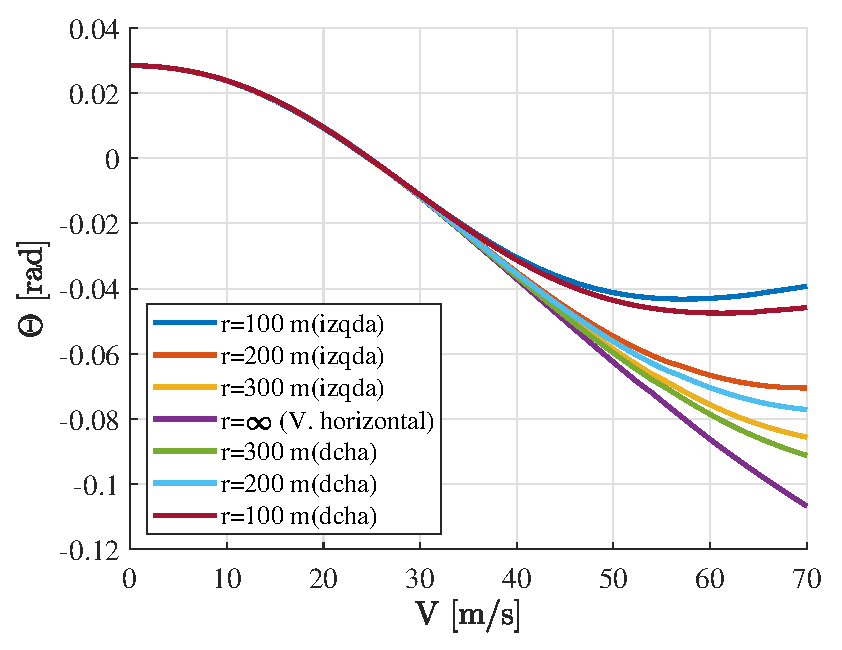
\includegraphics[width=90mm]{graficos/CabVCcs}
	\caption{Ángulo de cabeceo de la aeronave en función de la velocidad de vuelo a una altitud de 1000 m para vuelo circular de diferentes radios.}
	\label{CabVCcs}
\end{figure}
\begin{figure}
	\centering
	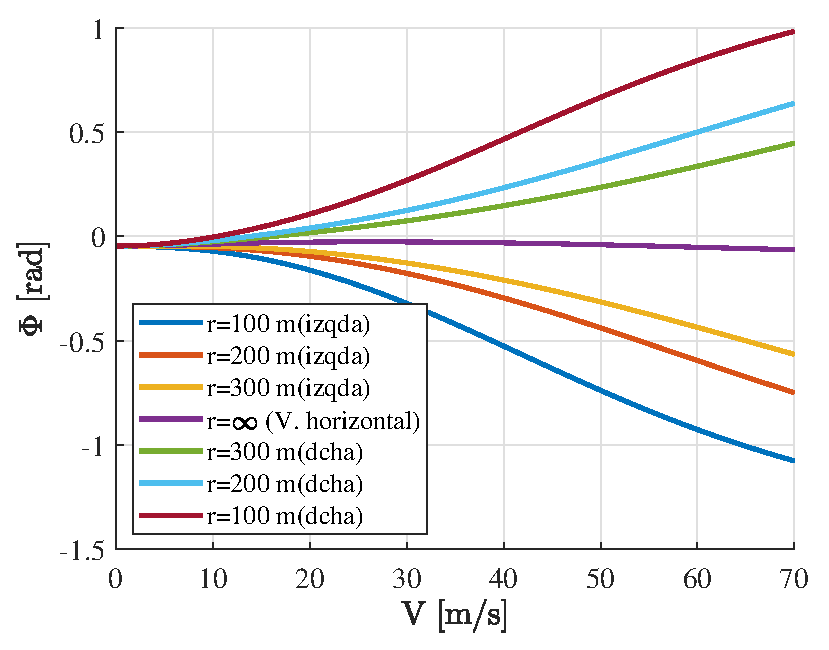
\includegraphics[width=90mm]{graficos/BalanVCcs}
	\caption{Ángulo de balanceo de la aeronave en función de la velocidad de vuelo a una altitud de 1000 m para vuelo circular de diferentes radios.}
	\label{BalanVCcs}
\end{figure}

En el caso del cabeceo (gráfica \ref{CabVCcs}) la evolución es la misma que vista anteriormente, solo que, en valor absoluto, el ángulo de cabeceo disminuye con el radio de la trayectoria, existiendo eso si en este caso mayores diferencias para los distintos sentidos de giro.

Sin embargo, en la gráfica \ref{BalanVCcs} es en la que los datos para un mismo radio y diferentes sentidos de giro están separados. Este resultado es obvio, ya que la gráfica corresponde al ángulo de balanceo. La aeronave tenderá a un valor de balanceo tal que las fuerzas del rotor tiendan hacia el sentido de giro para poder así efectuar la trayectoria.

De estos resultados se puede obtener una conclusión muy clara, para trayectorias de gran radio no se ha de tener especial cuidado, pero si se quieren recorrer trayectorias de menor radio, se ha de tener en cuenta que las actuaciones se verán mermadas, y que de ser posible conviene siempre diseñar las trayectorias con giros hacia la izquierda.

%\subsection*{Vuelo con Diferentes Cargas de Pago de Posición Variable}
%
%En capítulos anteriores se han definido las cargas de pago modelo y se han realizado ensayos numéricos acerca de su efecto en los distintos vuelos expuestos. Este apartado pretende abordar el mismo problema de manera breve, comentando los resultados más llamativos respecto a los anteriores análisis.
%
%\begin{figure}
%	\centering
%	\subfigure[Potencia necesaria para el vuelo en función de la posición relativa a $O_f$ de la carga 2 para una velocidad de vuelo de 10 m/s.]{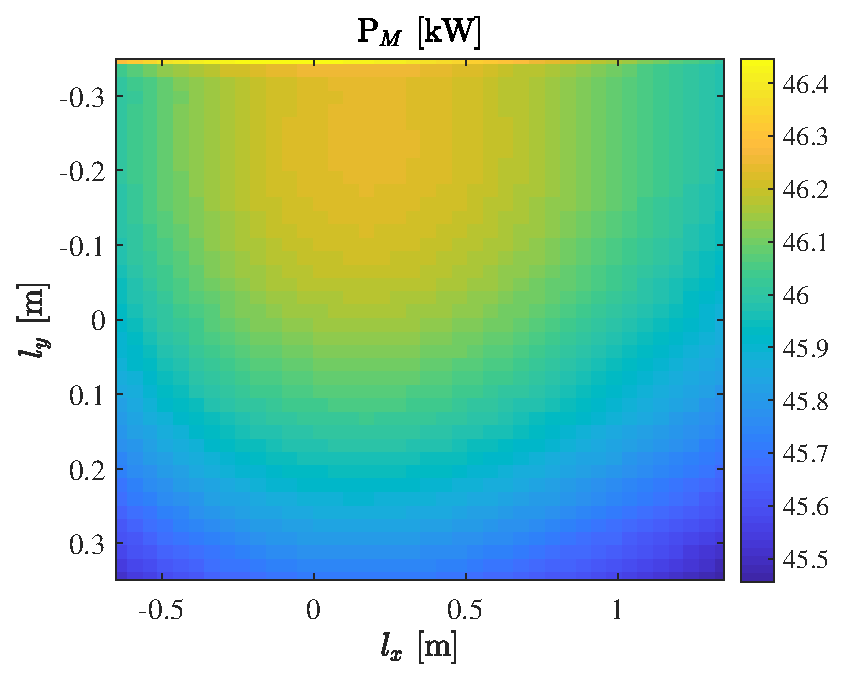
\includegraphics[width=60mm]{graficos/PMVC2lxy10ms}}
%	\subfigure[Potencia necesaria para el vuelo en función de la posición relativa a $O_f$ de la carga 2 para una velocidad de vuelo de 50 m/s.]{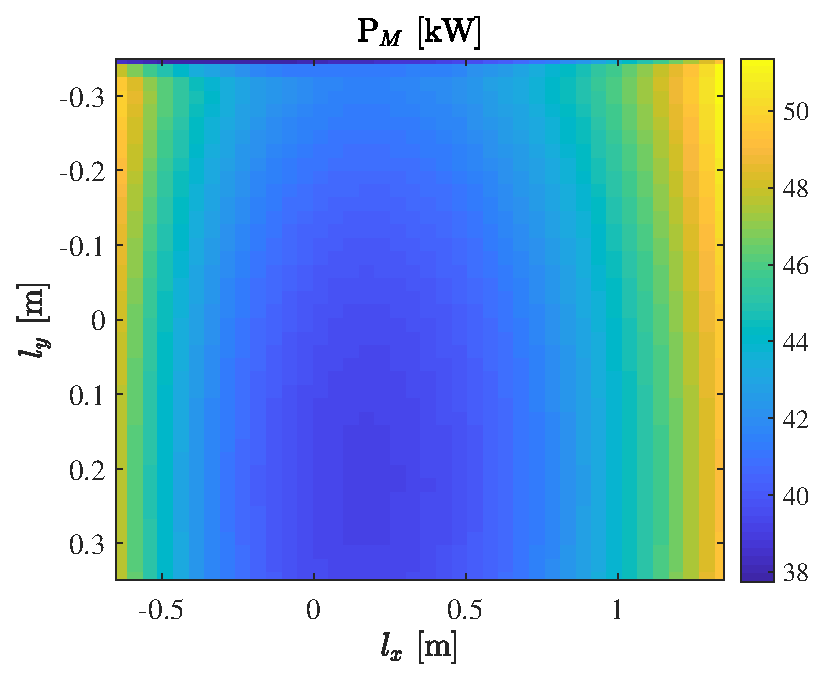
\includegraphics[width=60mm]{graficos/PMVC2lxy50ms}}
%	\caption{Consumo de Potencia de la aeronave en función de la posición relativa a $O_f$ de la carga 2.}
%	\label{PMVC2lxy}
%\end{figure}
%\begin{figure}
%	\centering
%	\subfigure[Potencia necesaria para el vuelo en función de la posición relativa a $O_f$ de la carga 3 para una velocidad de vuelo de 10 m/s.]{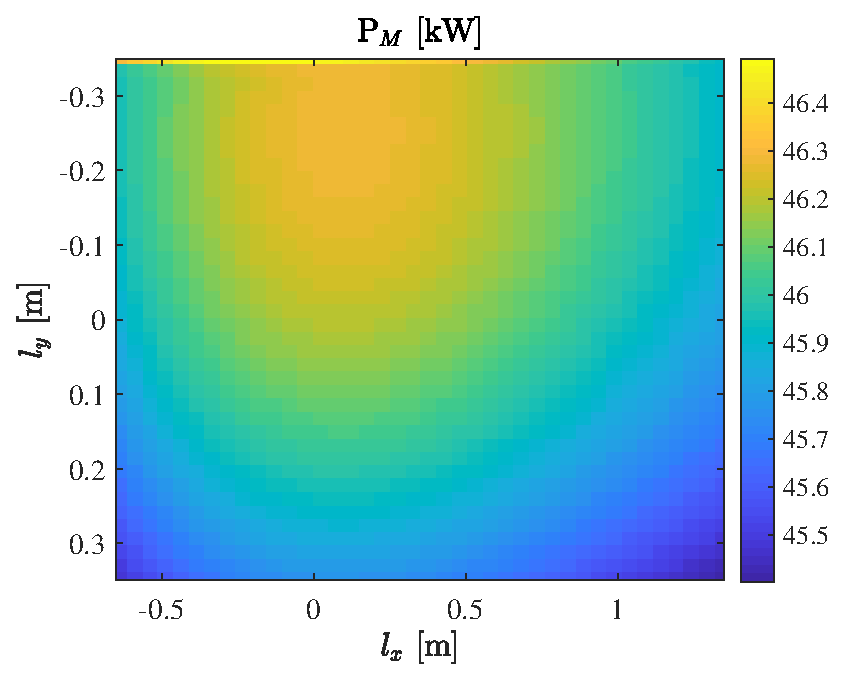
\includegraphics[width=60mm]{graficos/PMVC3lxy10ms}}
%	\subfigure[Potencia necesaria para el vuelo en función de la posición relativa a $O_f$ de la carga 3 para una velocidad de vuelo de 50 m/s.]{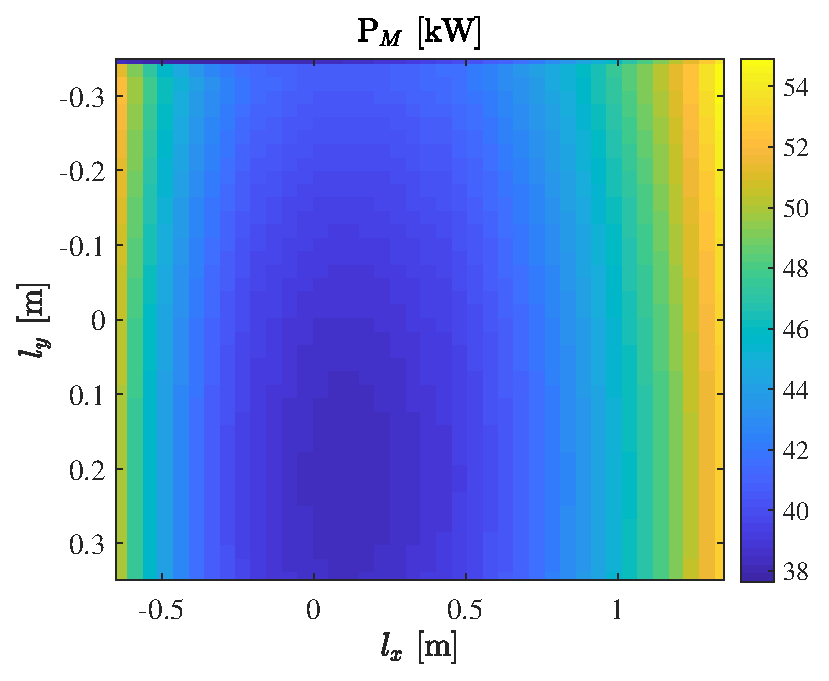
\includegraphics[width=60mm]{graficos/PMVC3lxy50ms}}
%	\caption{Consumo de Potencia de la aeronave en función de la posición relativa a $O_f$ de la carga 3.}
%	\label{PMVC3lxy}
%\end{figure}
%\begin{figure}
%	\centering
%	\subfigure[Ángulo de paso colectivo del rotor principal en función de la posición relativa a $O_f$ de la carga 2 para una velocidad de vuelo de 10 m/s.]{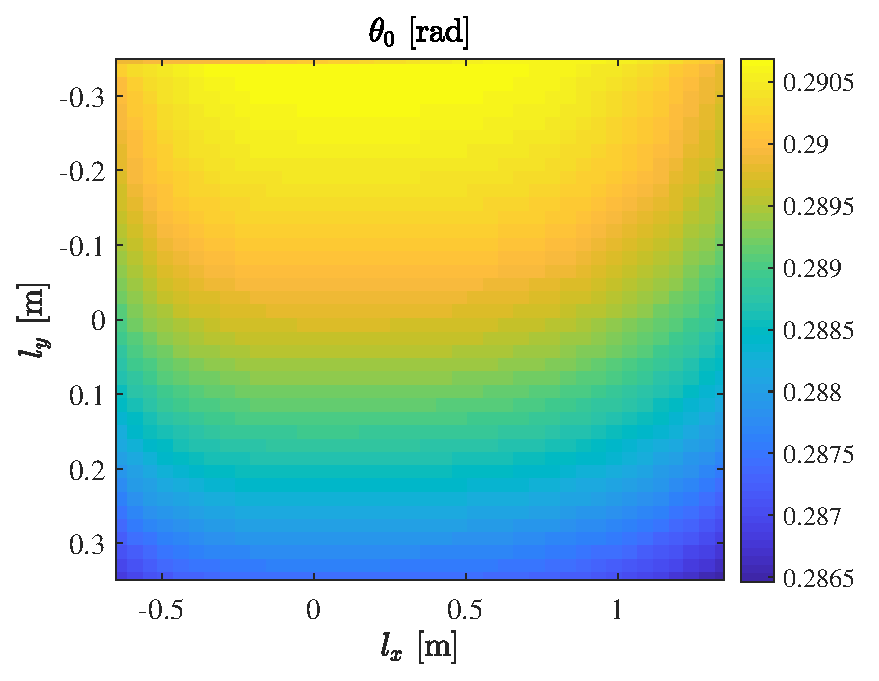
\includegraphics[width=60mm]{graficos/theta0VC2lxy10ms}}
%	\subfigure[Ángulo de paso colectivo del rotor principal en función de la posición relativa a $O_f$ de la carga 2 para una velocidad de vuelo de 50 m/s.]{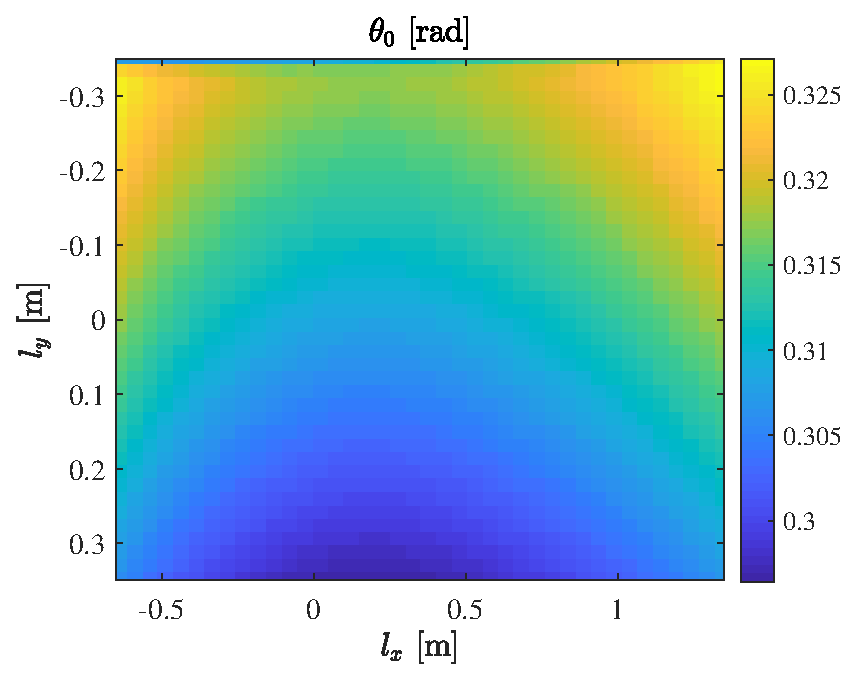
\includegraphics[width=60mm]{graficos/theta0VC2lxy50ms}}
%	\caption{Ángulo de paso colectivo del rotor principal en función de la posición relativa a $O_f$ de la carga 2.}
%	\label{theta0VC2lxy}
%\end{figure}
%\begin{figure}
%	\centering
%	\subfigure[Ángulo de paso colectivo del rotor principal en función de la posición relativa a $O_f$ de la carga 3 para una velocidad de vuelo de 10 m/s.]{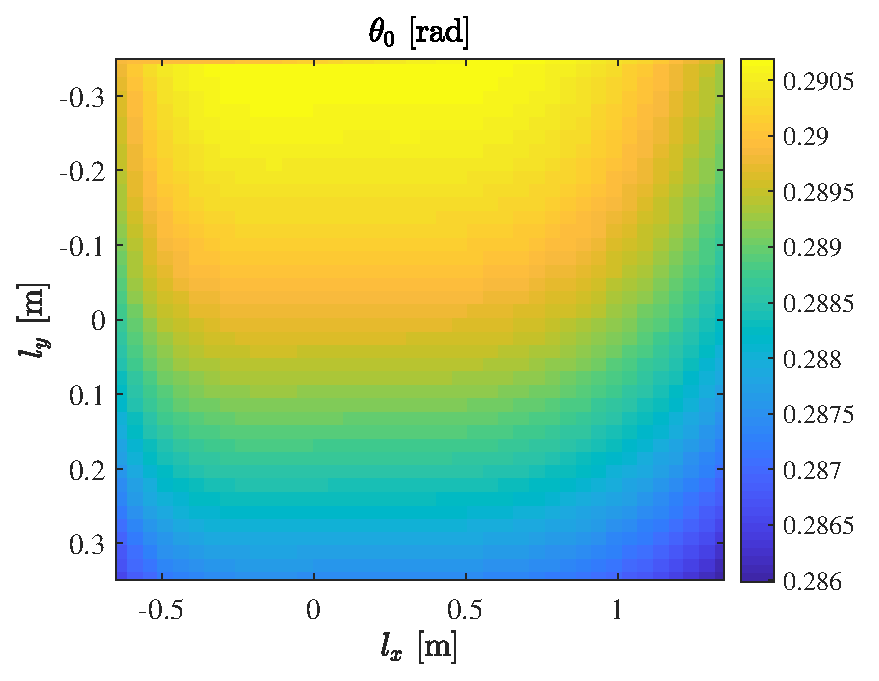
\includegraphics[width=60mm]{graficos/theta0VC3lxy10ms}}
%	\subfigure[Ángulo de paso colectivo del rotor principal en función de la posición relativa a $O_f$ de la carga 3 para una velocidad de vuelo de 50 m/s.]{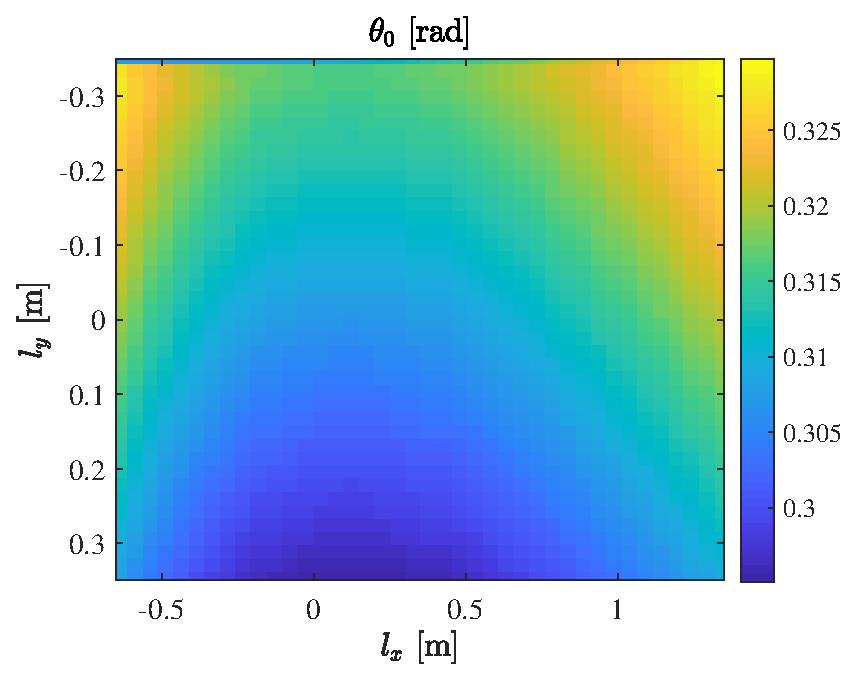
\includegraphics[width=60mm]{graficos/theta0VC3lxy50ms}}
%	\caption{Ángulo de paso colectivo del rotor principal en función de la posición relativa a $O_f$ de la carga 3.}
%	\label{theta0VC3lxy}
%\end{figure}
%\begin{figure}
%	\centering
%	\subfigure[Ángulo de paso cíclico longitudinal en función de la posición relativa a $O_f$ de la carga 2 para una velocidad de vuelo de 10 m/s.]{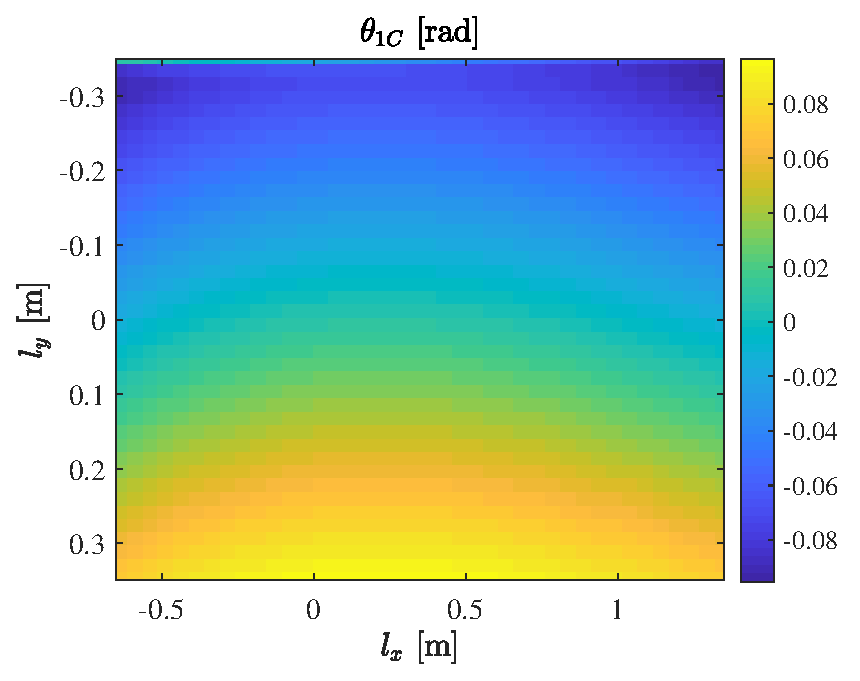
\includegraphics[width=60mm]{graficos/theta1CVC2lxy10ms}}
%	\subfigure[Ángulo de paso cíclico longitudinal en función de la posición relativa a $O_f$ de la carga 2 para una velocidad de vuelo de 50 m/s.]{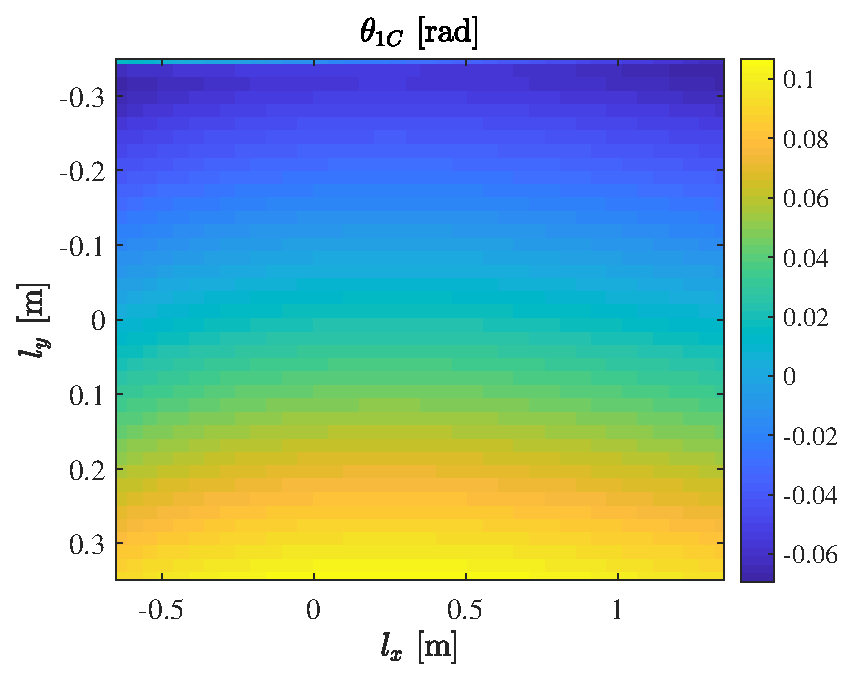
\includegraphics[width=60mm]{graficos/theta1CVC2lxy50ms}}
%	\caption{Ángulo de paso cíclico longitudinal en función de la posición relativa a $O_f$ de la carga 2.}
%	\label{theta1CVC2lxy}
%\end{figure}
%\begin{figure}
%	\centering
%	\subfigure[Ángulo de paso cíclico longitudinal en función de la posición relativa a $O_f$ de la carga 3 para una velocidad de vuelo de 10 m/s.]{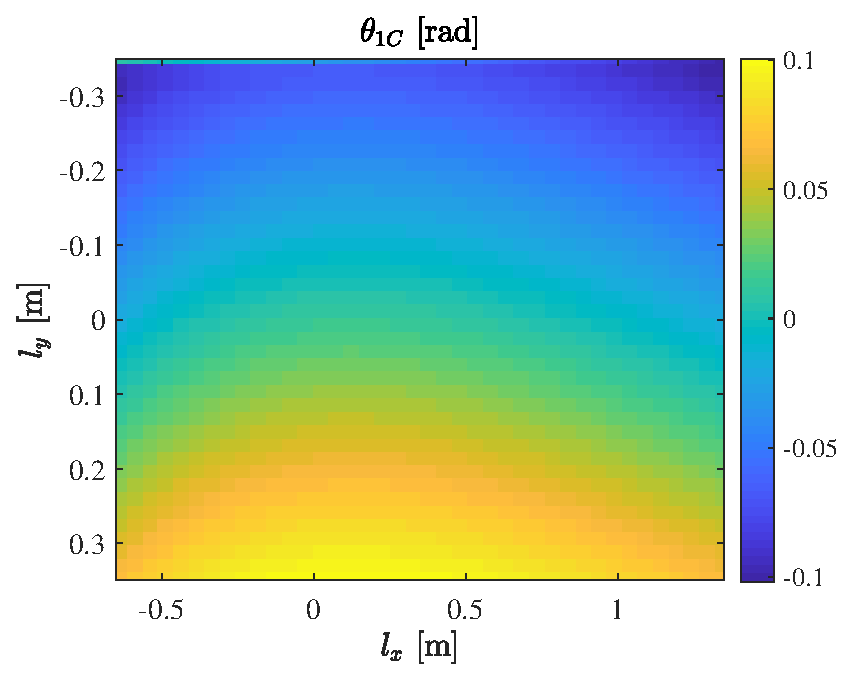
\includegraphics[width=60mm]{graficos/theta1CVC3lxy10ms}}
%	\subfigure[Ángulo de paso cíclico longitudinal en función de la posición relativa a $O_f$ de la carga 3 para una velocidad de vuelo de 50 m/s.]{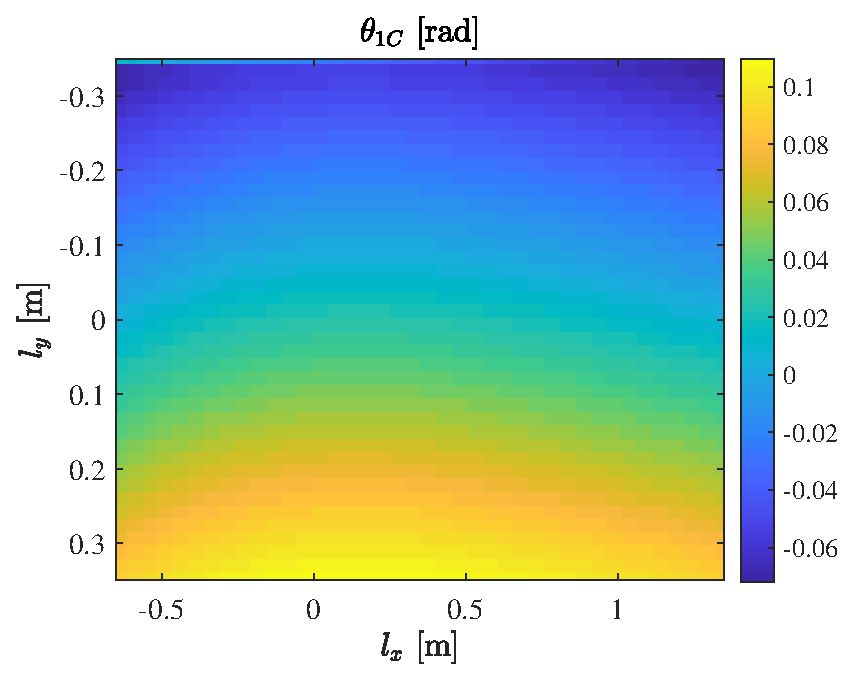
\includegraphics[width=60mm]{graficos/theta1CVC3lxy50ms}}
%	\caption{Ángulo de paso cíclico longitudinal en función de la posición relativa a $O_f$ de la carga 3.}
%	\label{theta1CVC3lxy}
%\end{figure}
%\begin{figure}
%	\centering
%	\subfigure[Ángulo de paso cíclico lateral en función de la posición relativa a $O_f$ de la carga 2 para una velocidad de vuelo de 10 m/s.]{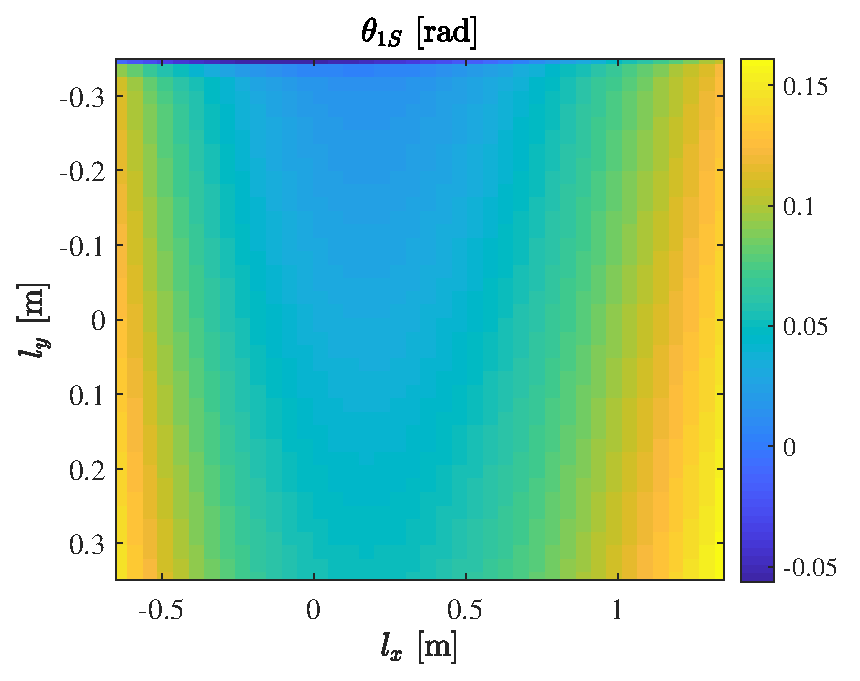
\includegraphics[width=60mm]{graficos/theta1SVC2lxy10ms}}
%	\subfigure[Ángulo de paso cíclico lateral en función de la posición relativa a $O_f$ de la carga 2 para una velocidad de vuelo de 50 m/s.]{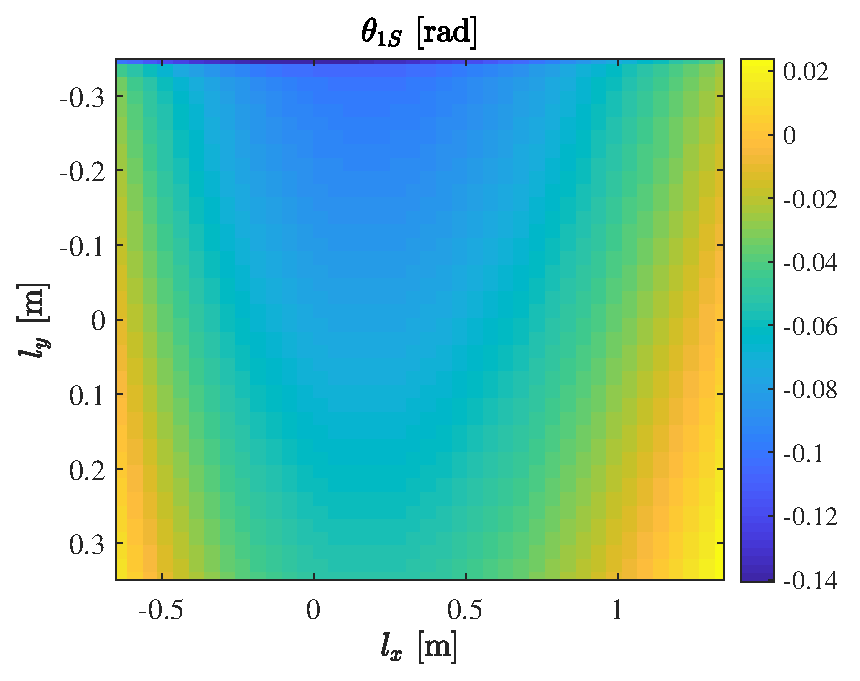
\includegraphics[width=60mm]{graficos/theta1SVC2lxy50ms}}
%	\caption{Ángulo de paso cíclico lateral en función de la posición relativa a $O_f$ de la carga 2.}
%	\label{theta1SVC2lxy}
%\end{figure}
%\begin{figure}
%	\centering
%	\subfigure[Ángulo de paso cíclico lateral en función de la posición relativa a $O_f$ de la carga 3 para una velocidad de vuelo de 10 m/s.]{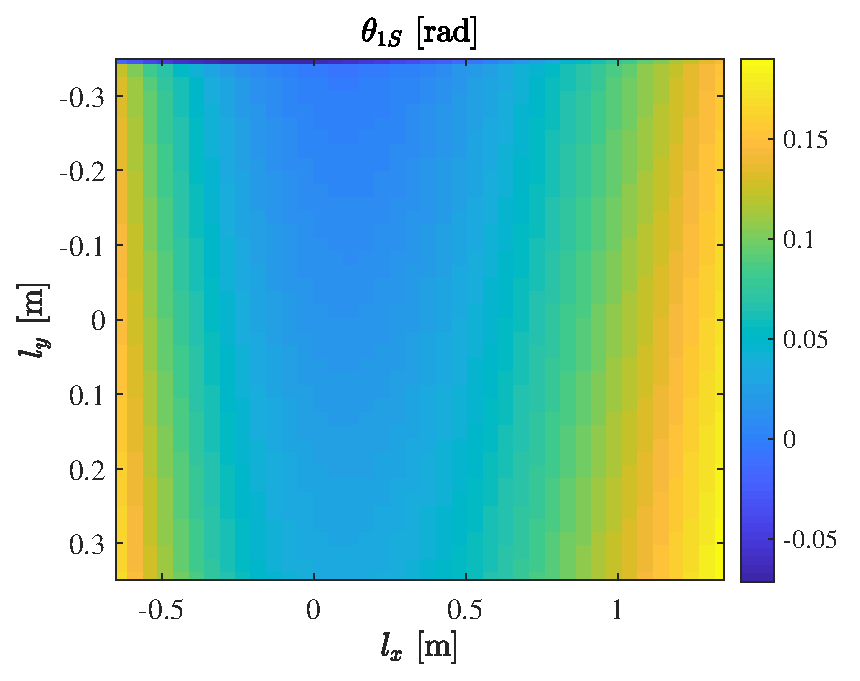
\includegraphics[width=60mm]{graficos/theta1SVC3lxy10ms}}
%	\subfigure[Ángulo de paso cíclico lateral en función de la posición relativa a $O_f$ de la carga 3 para una velocidad de vuelo de 50 m/s.]{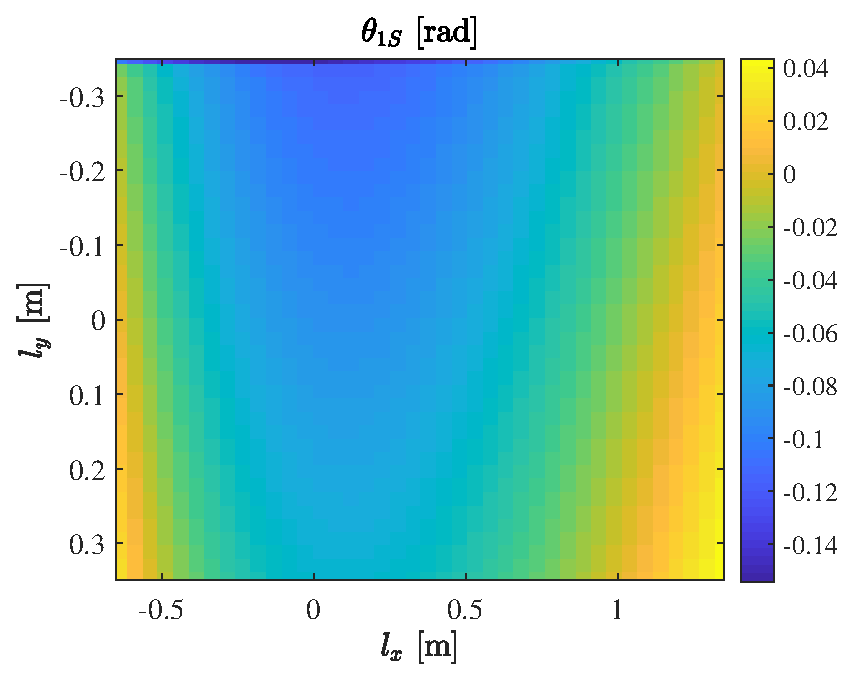
\includegraphics[width=60mm]{graficos/theta1SVC3lxy50ms}}
%	\caption{Ángulo de paso cíclico lateral en función de la posición relativa a $O_f$ de la carga 3.}
%	\label{theta1SVC3lxy}
%\end{figure}
%\begin{figure}
%	\centering
%	\subfigure[Ángulo de cabeceo de la aeronave en función de la posición relativa a $O_f$ de la carga 2 para una velocidad de vuelo de 10 m/s.]{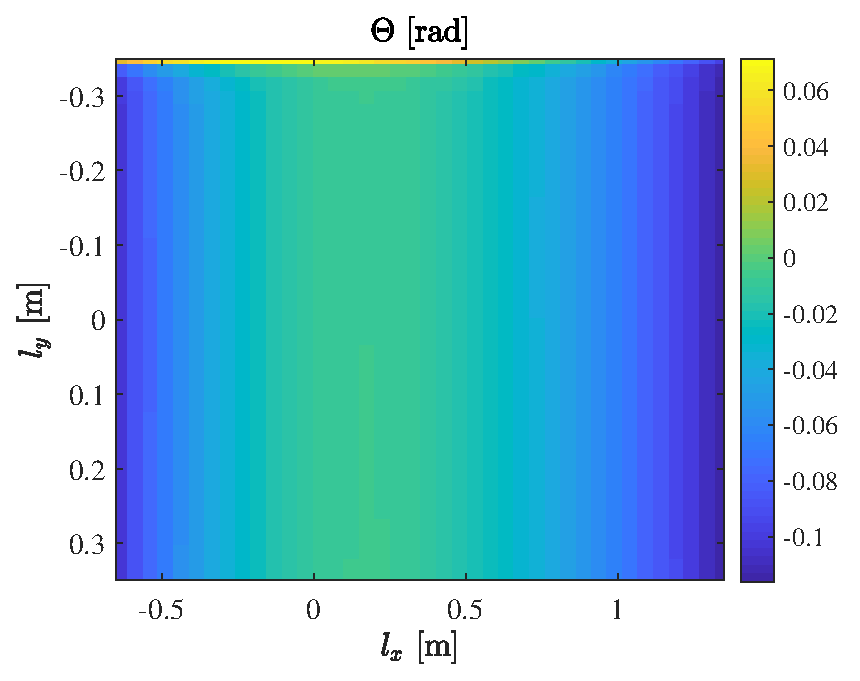
\includegraphics[width=60mm]{graficos/CabVC2lxy10ms}}
%	\subfigure[Ángulo de cabeceo de la aeronave en función de la posición relativa a $O_f$ de la carga 2 para una velocidad de vuelo de 50 m/s.]{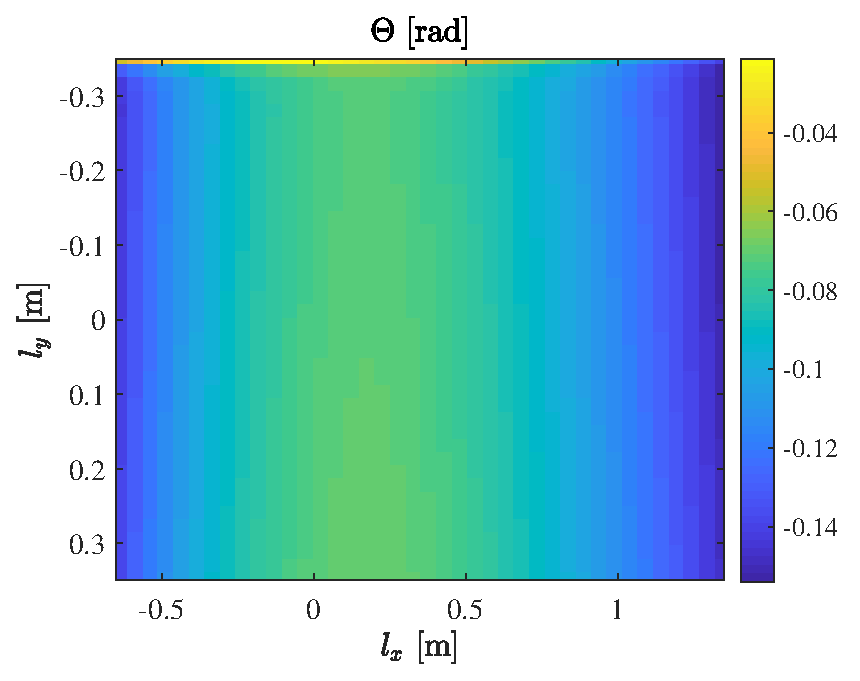
\includegraphics[width=60mm]{graficos/CabVC2lxy50ms}}
%	\caption{Ángulo de cabeceo de la aeronave en función de la posición relativa a $O_f$ de la carga 2.}
%	\label{CabVC2lxy}
%\end{figure}
%\begin{figure}
%	\centering
%	\subfigure[Ángulo de cabeceo de la aeronave en función de la posición relativa a $O_f$ de la carga 3 para una velocidad de vuelo de 10 m/s.]{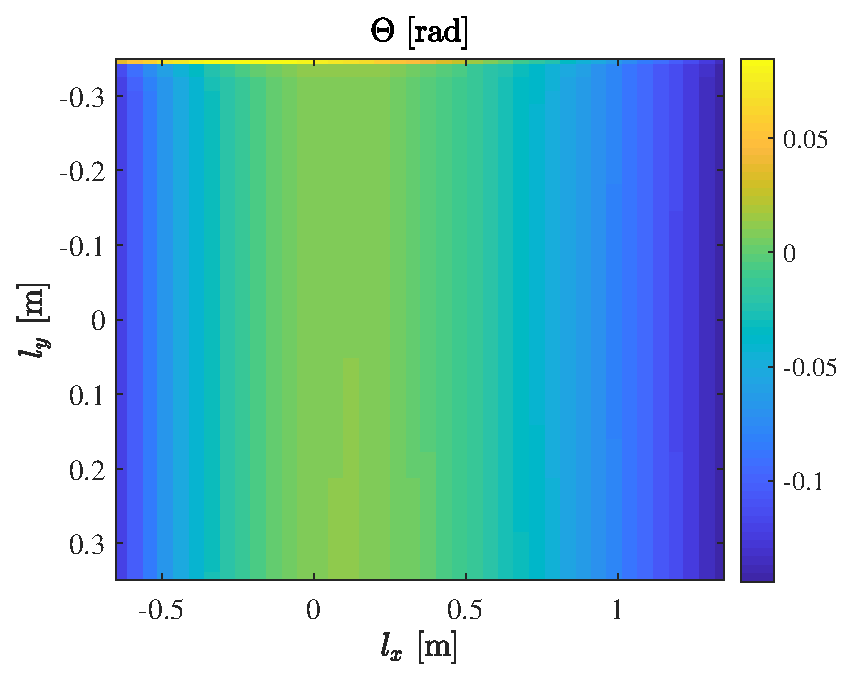
\includegraphics[width=60mm]{graficos/CabVC3lxy10ms}}
%	\subfigure[Ángulo de cabeceo de la aeronave en función de la posición relativa a $O_f$ de la carga 3 para una velocidad de vuelo de 50 m/s.]{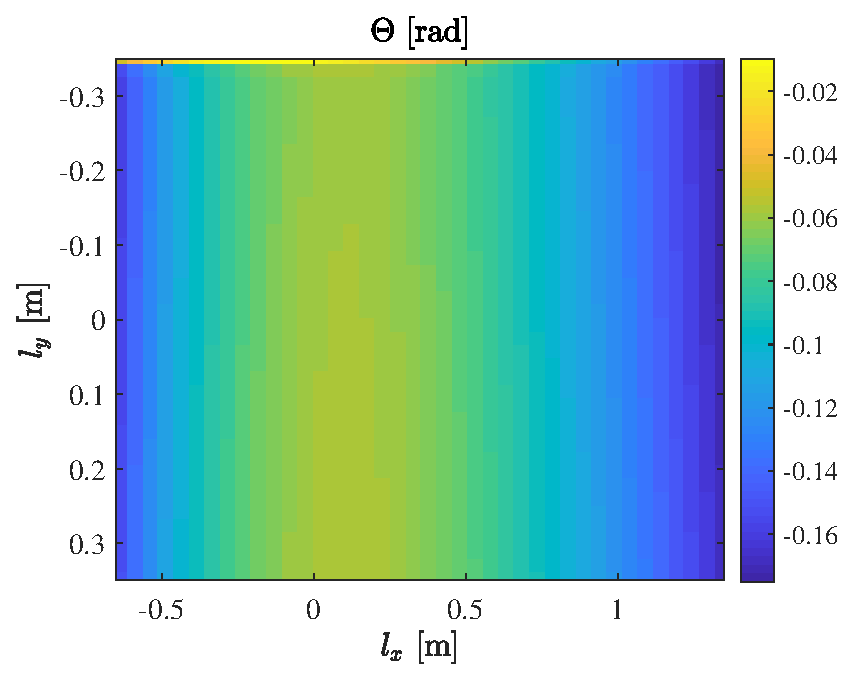
\includegraphics[width=60mm]{graficos/CabVC3lxy50ms}}
%	\caption{Ángulo de cabeceo de la aeronave en función de la posición relativa a $O_f$ de la carga 3.}
%	\label{CabVC3lxy}
%\end{figure}
%
%\begin{figure}
%	\centering
%	\subfigure[Ángulo de balanceo de la aeronave en función de la posición relativa a $O_f$ de la carga 2 para una velocidad de vuelo de 10 m/s.]{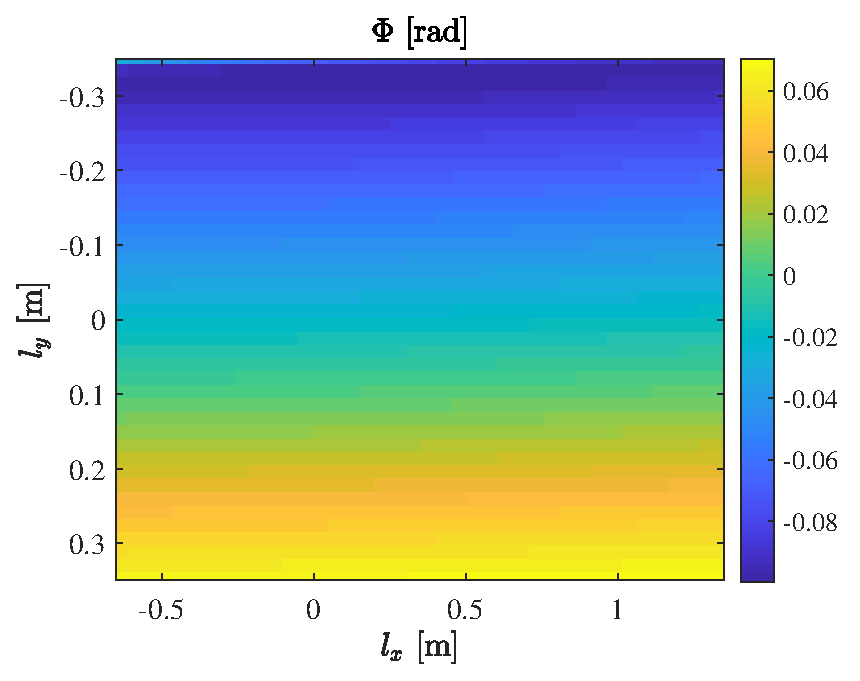
\includegraphics[width=60mm]{graficos/BalanVC2lxy10ms}}
%	\subfigure[Ángulo de balanceo de la aeronave en función de la posición relativa a $O_f$ de la carga 2 para una velocidad de vuelo de 50 m/s.]{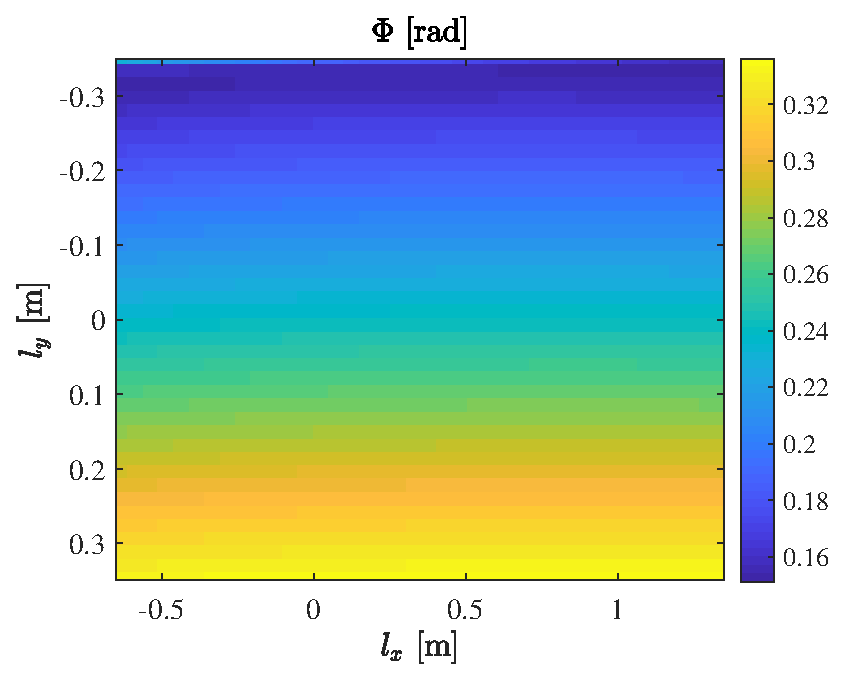
\includegraphics[width=60mm]{graficos/BalanVC2lxy50ms}}
%	\caption{Ángulo de balanceo de la aeronave en función de la posición relativa a $O_f$ de la carga 2.}
%	\label{BalanVC2lxy}
%\end{figure}
%\begin{figure}
%	\centering
%	\subfigure[Ángulo de balanceo de la aeronave en función de la posición relativa a $O_f$ de la carga 3 para una velocidad de vuelo de 10 m/s.]{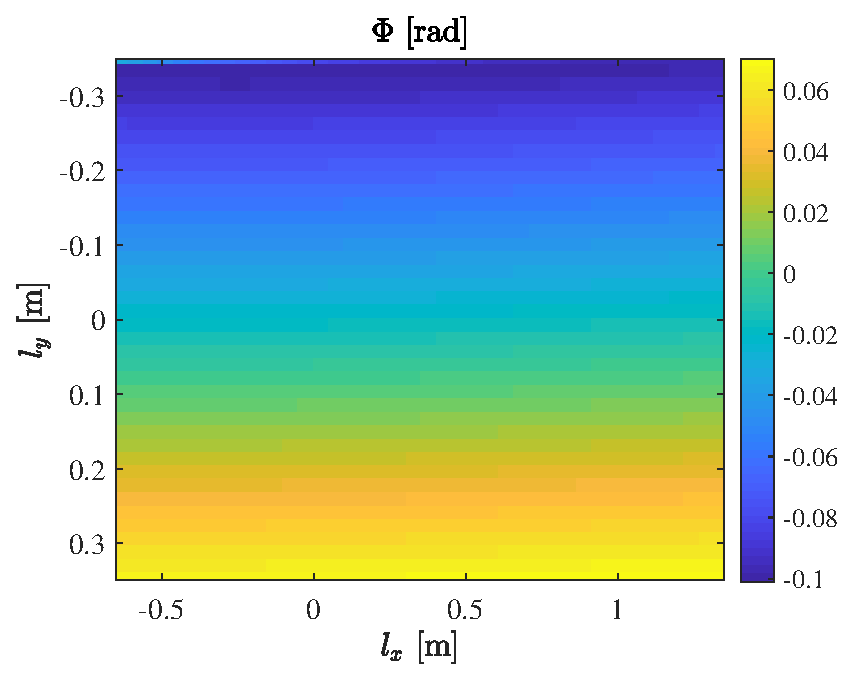
\includegraphics[width=60mm]{graficos/BalanVC3lxy10ms}}
%	\subfigure[Ángulo de balanceo de la aeronave en función de la posición relativa a $O_f$ de la carga 3 para una velocidad de vuelo de 50 m/s.]{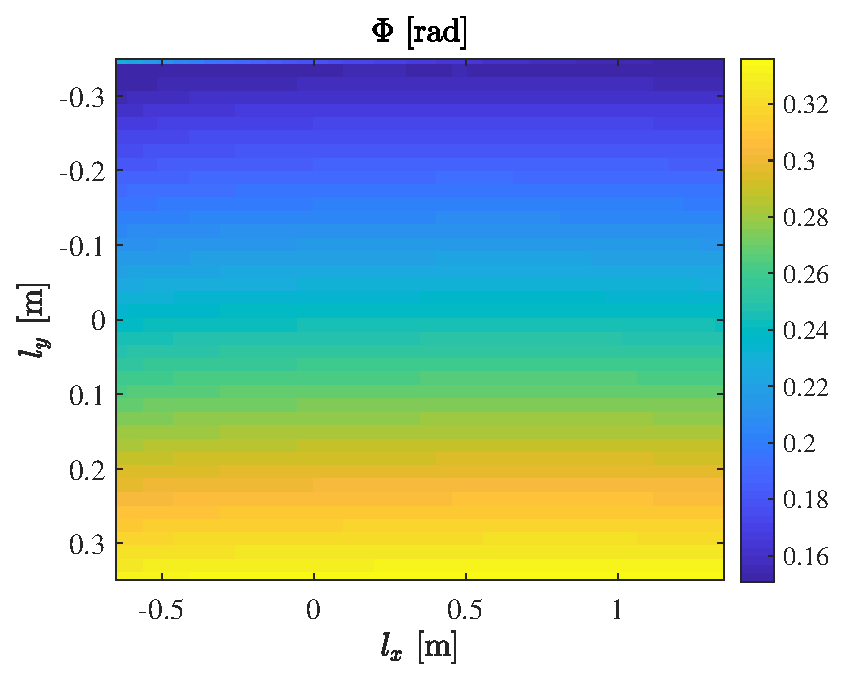
\includegraphics[width=60mm]{graficos/BalanVC3lxy50ms}}
%	\caption{Ángulo de balanceo de la aeronave en función de la posición relativa a $O_f$ de la carga 3.}
%	\label{BalanVC3lxy}
%\end{figure}
%\begin{figure}
%	\centering
%	\subfigure[Ángulo de paso colectivo del rotor antipar en función de la posición relativa a $O_f$ de la carga 2 para una velocidad de vuelo de 10 m/s.]{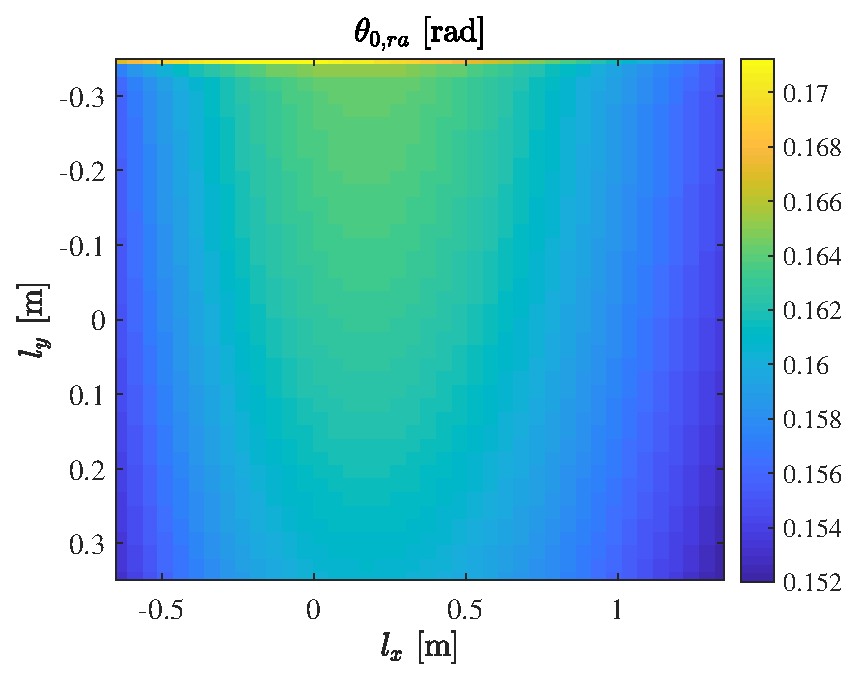
\includegraphics[width=60mm]{graficos/theta0raVC2lxy10ms}}
%	\subfigure[Ángulo de paso colectivo del rotor antipar en función de la posición relativa a $O_f$ de la carga 2 para una velocidad de vuelo de 50 m/s.]{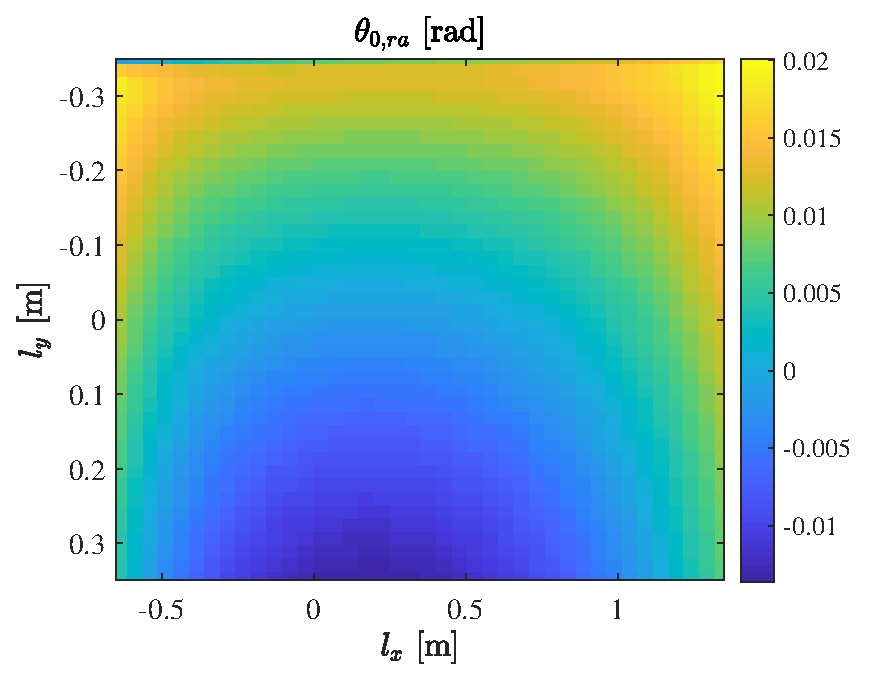
\includegraphics[width=60mm]{graficos/theta0raVC2lxy50ms}}
%	\caption{Ángulo de paso colectivo del rotor antipar en función de la posición relativa a $O_f$ de la carga 2.}
%	\label{theta0raVC2lxy}
%\end{figure}
%\begin{figure}
%	\centering
%	\subfigure[Ángulo de paso colectivo del rotor antipar en función de la posición relativa a $O_f$ de la carga 3 para una velocidad de vuelo de 10 m/s.]{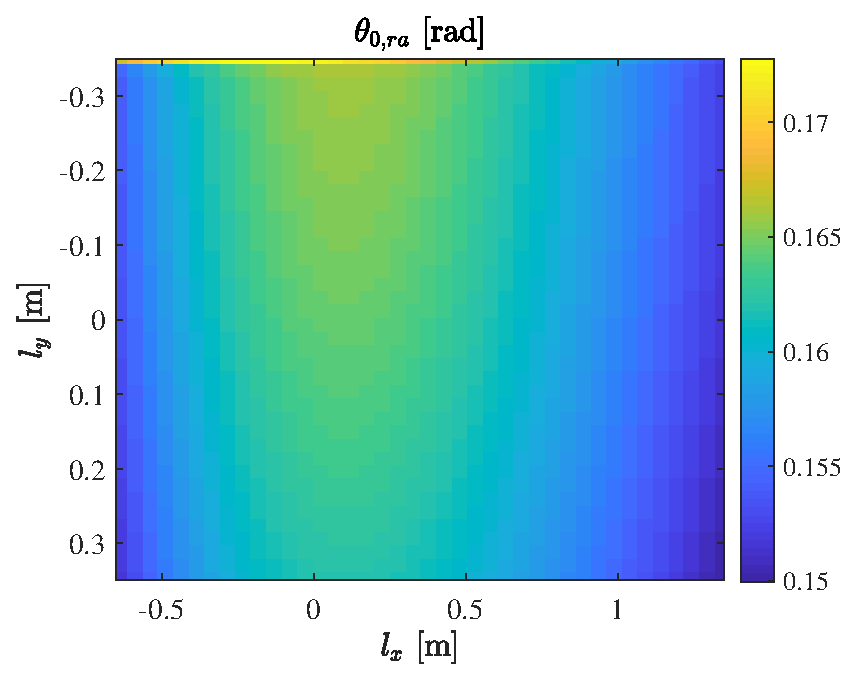
\includegraphics[width=60mm]{graficos/theta0raVC3lxy10ms}}
%	\subfigure[Ángulo de paso colectivo del rotor antipar en función de la posición relativa a $O_f$ de la carga 3 para una velocidad de vuelo de 50 m/s.]{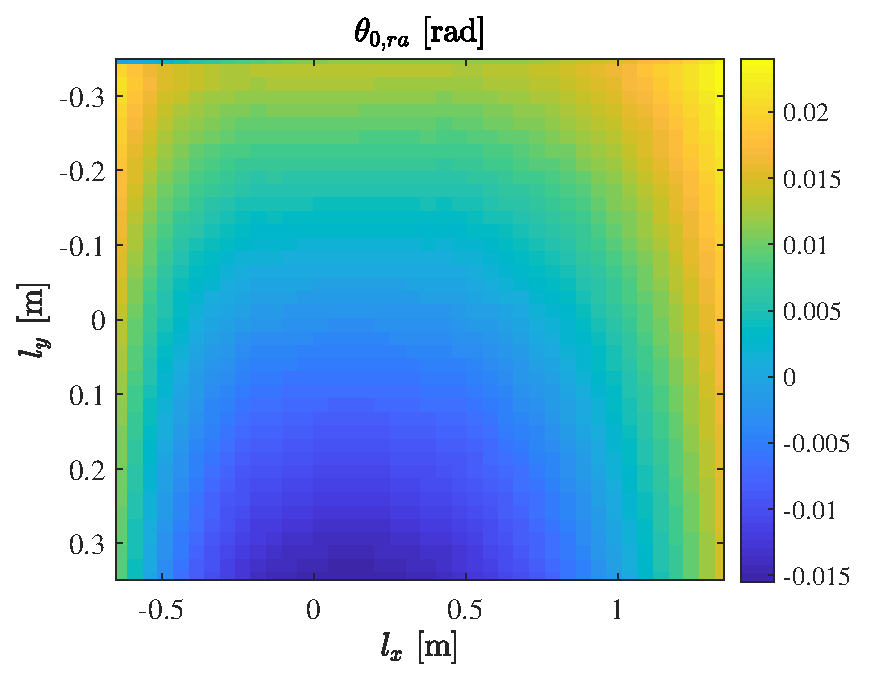
\includegraphics[width=60mm]{graficos/theta0raVC3lxy50ms}}
%	\caption{Ángulo de paso colectivo del rotor antipar en función de la posición relativa a $O_f$ de la carga 3.}
%	\label{theta0raVC3lxy}
%\end{figure}



\subsection*{Triple Carga de Pago con Restricciones a la Posición}

En un principio se pensó añadir el análisis de los parámetros de vuelo en función de la posición de la carga, pero los resultados eran prácticamente idénticos a dados en el vuelo horizontal, por lo que su análisis resultaba irrelevante.
Por ello, como último ensayo, se ha querido representar una situación fuera de lo común para comprobar como respondería la aeronave. Dicha situación consiste en lo siguiente:

\begin{itemize}
	\item El helicóptero lleva embarcadas dos cargas de pago:
	\subitem Carga 2 en una posición tal que $l_x=1.3$ m y $l_y=0.3$ m.
	\subitem Carga 3 en una posición tal que $l_x=1.25$ m y $l_y=-0.25$ m.
	\item El vuelo a realizar es circular, de radio 300 m a una altitud de 1000 m y una velocidad de 30 m/s.
\end{itemize}
El usuario requiere embarcar una última carga de pago especial que se denominará "carga 4" y cuyos datos están recogidos en la tabla \ref{carga4}. Se puede apreciar que no tiene una posición fija, ya que en cualquier posición que cumpla los requisitos de la tabla, la carga podrá llevar a cabo su misión.
El objetivo de este análisis es comprobar dónde sería más conveniente colocar la carga 4 para mantener o mejorar los parámetros del vuelo.
Cabe destacar que se considera que la implementación de cada carga permite reducir algún sistema de a bordo del mismo peso que la carga y cuyo centro de masas coincidía con el de la aeronave, de manera que la masa total al despegue siempre es de 450 kg y el centro de gravedad de la aeronave en sin las cargas no se ve alterado.

\begin{table}[htbp]
	\centering
	\begin{tabular}{|>{\columncolor{Gray}}c|c|}
		\hline
		\cellcolor{Gray}Masa del dispositivo ($M_{pl}$) & 50 kg \\ \hline
		\cellcolor{Gray}Radio del dispositivo ($R_{pl}$) & 0.2 m \\ \hline
		\cellcolor{Gray}Momento de inercia del eje $x$ ($I_{x}^{pl0}$) & 0.8 kg$\cdot$m$^2$ \\ \hline
		\cellcolor{Gray}Momento de inercia del eje $y$ ($I_{y}^{pl0}$) & 0.8 kg$\cdot$m$^2$ \\ \hline
		\cellcolor{Gray}Momento de inercia del eje $z$ ($I_{z}^{pl0}$) & 0.8 kg$\cdot$m$^2$ \\ \hline
		\cellcolor{Gray}Producto de inercia $xy$ ($I_{xy}^{pl0}$)& 0 kg$\cdot$m$^2$ \\ \hline
		\cellcolor{Gray}Producto de inercia $xz$ ($I_{xz}^{pl0}$)& 0 kg$\cdot$m$^2$ \\ \hline
		\cellcolor{Gray}Producto de inercia $yz$ ($I_{yz}^{pl0}$)& 0 kg$\cdot$m$^2$ \\ \hline
		\cellcolor{Gray}Peso del dispositivo ($W_{pl}$)& 50$\cdot$9.81 N \\ \hline
		\cellcolor{Gray}Posición longitudinal de la carga de pago respecto a $O_f$ ($l_x$) & [-0.1 1] m \\ \hline
		\cellcolor{Gray}Posición transversal de la carga de pago respecto a $O_f$ ($l_y$) & [-0.4 0.4] m \\ \hline
		\cellcolor{Gray}Posición vertical del suelo del fuselaje ($l_z$) & 0.7678 m \\ \hline
	\end{tabular}%
	\caption{Valores másicos, de inercia y de posición de la carga de pago "carga 4".}
	\label{carga4}
\end{table}%
\subsubsection*{Efectos de la Integración de la Carga}

Primero se procederá a comparar las características del vuelo para el vehículo con y sin la carga 4 embarcada en la posición $l_x=0.4$ m y $l_y=-0.1$ m, suponiendo como en los casos anteriores que el peso total de la aeronave es de 450 kg.

\begin{figure}
	\centering
	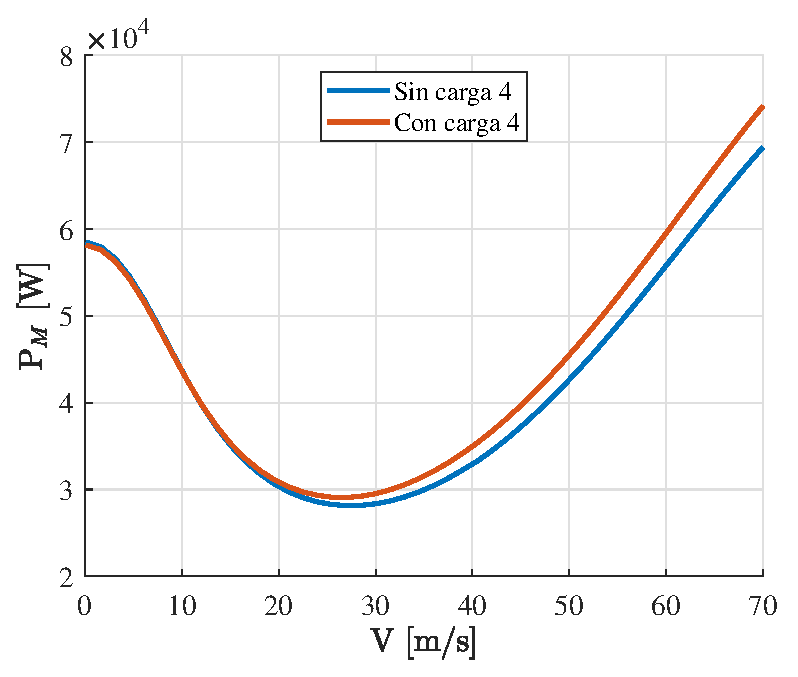
\includegraphics[width=90mm]{graficos/PMVCSP}
	\caption{Consumo de Potencia de la aeronave con y sin carga 4 embarcada en $l_x=0.4$ m y $l_y=-0.1$ m en función de la velocidad a 1000 m de altitud y vuelo circular de radio 300 m.}
	\label{PMVCSP}
\end{figure}

Lo primero que se aprecia en la gráfica \ref{PMVCSP} es que la potencia necesaria para el vuelo se incrementa con la carga para altas velocidades, reduciéndose la velocidad máxima en esas condiciones de 61.6 m/s a 59 m/s. Para muy bajas velocidades, esta relación se invierte, reduciéndose el consumo de potencia con la implementación de la carga, aunque de manera ínfima. El ángulo de paso colectivo del rotor principal, representado en la gráfica \ref{Theta0VCSP}, sufre una evolución similar, solo que el incremento de valor del paso para velocidades cercanas a los 55 m/s es de 0.004 rad.
\begin{figure}
	\centering
	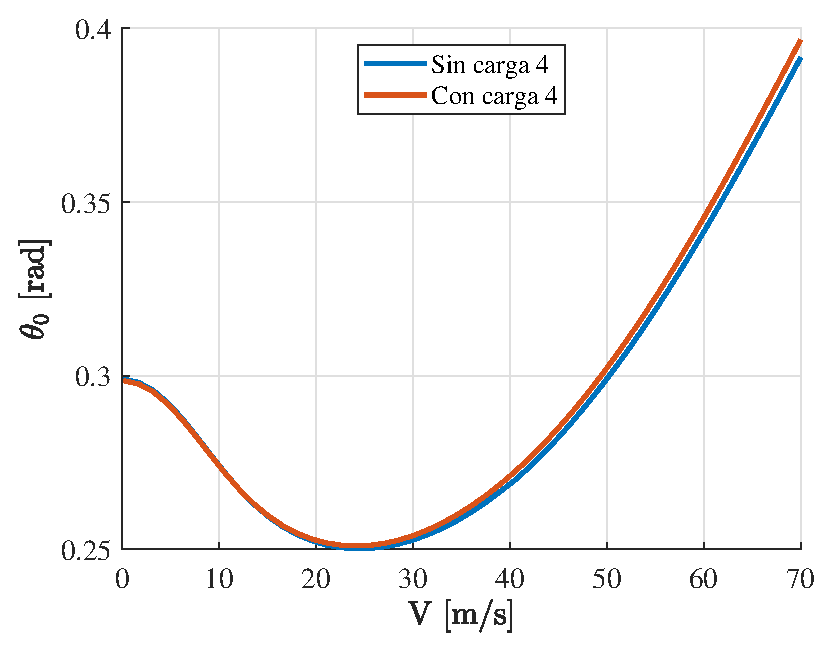
\includegraphics[width=90mm]{graficos/theta0VCSP}
	\caption{Ángulos de paso colectivo del rotor principal de la aeronave con y sin carga 4 embarcada en $l_x=0.4$ m y $l_y=-0.1$ m en función de la velocidad a 1000 m de altitud y vuelo circular de radio 300 m.}
	\label{Theta0VCSP}
\end{figure}
\begin{figure}
	\centering
	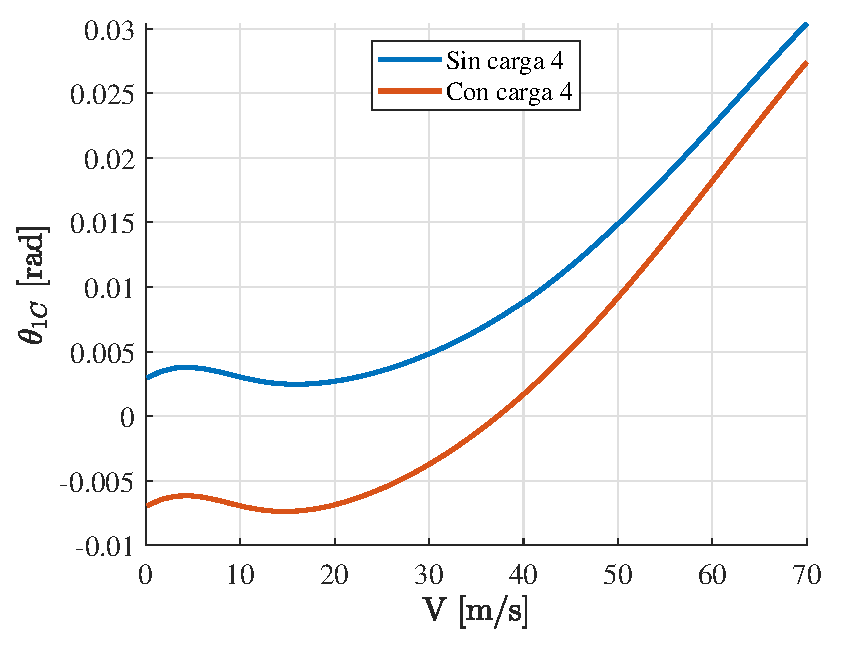
\includegraphics[width=90mm]{graficos/theta1CVCSP}
	\caption{Ángulos de paso cíclico longitudinal del rotor principal de la aeronave con y sin carga 4 embarcada en $l_x=0.4$ m y $l_y=-0.1$ m en función de la velocidad a 1000 m de altitud y vuelo circular de radio 300 m.}
	\label{Theta1CVCSP}
\end{figure}
Se puede apreciar en las gráficas \ref{Theta1CVCSP} y \ref{Theta1SVCSP} que las diferencias en los ángulos de paso cíclico son mayores a bajas velocidades, aumentando el paso lateral y disminuyendo el paso longitudinal (pasando a valores negativos) con la carga. En el caso del paso cíclico longitudinal, las diferencias alcanzan valores de 0.01 rad, mientras que en el del paso cíclico lateral, estas alcanzan valores de 0.04 rad.
\begin{figure}
	\centering
	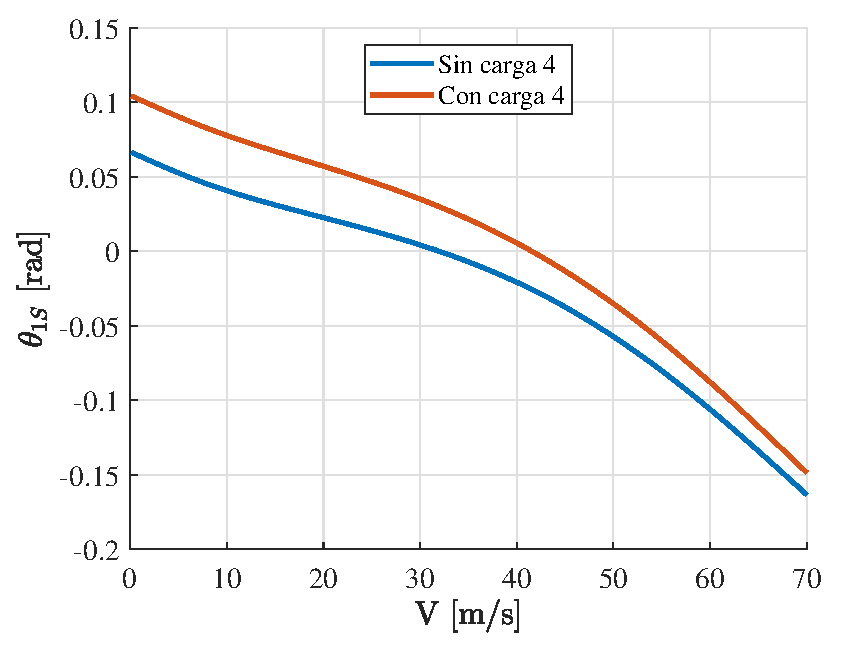
\includegraphics[width=90mm]{graficos/theta1SVCSP}
	\caption{Ángulos de paso cíclico lateral del rotor principal de la aeronave con y sin carga 4 embarcada en $l_x=0.4$ m y $l_y=-0.1$ m en función de la velocidad a 1000 m de altitud y vuelo circular de radio 300 m.}
	\label{Theta1SVCSP}
\end{figure}
\begin{figure}
	\centering
	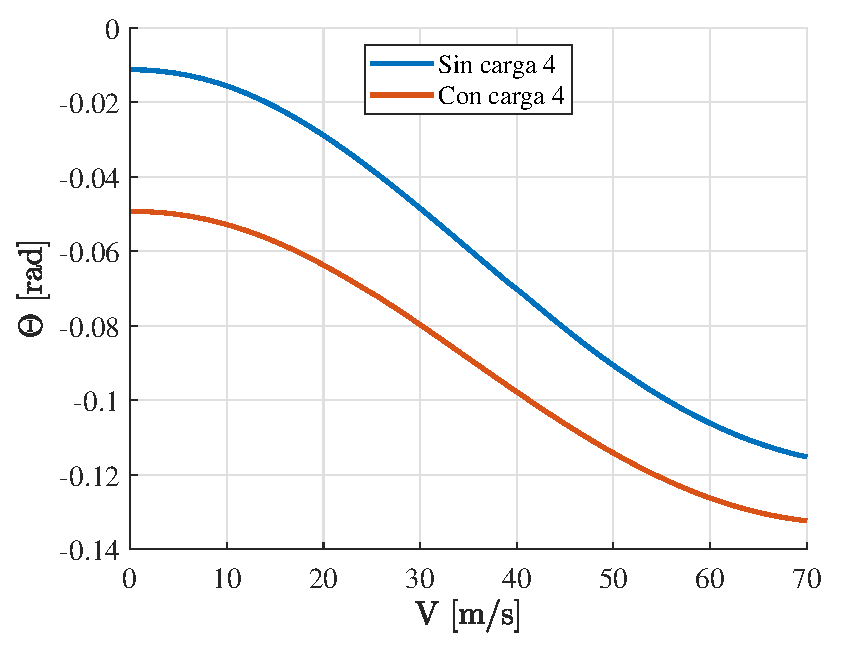
\includegraphics[width=90mm]{graficos/CabVCSP}
	\caption{Ángulos de cabeceo de la aeronave con y sin carga 4 embarcada en $l_x=0.4$ m y $l_y=-0.1$ m en función de la velocidad a 1000 m de altitud y vuelo circular de radio 300 m.}
	\label{ThetaVCSP}
\end{figure}

Respecto a los ángulos de Euler, la gráfica \ref{PhiVCSP} indica que el ángulo de balanceo se mantiene tras la instalación de la carga. Sin embargo, el desequilibrio másico longitudinal introducido por la carga provoca la disminución del ángulo de cabeceo de la aeronave, como se aprecia en la gráfica \ref{ThetaVCSP}. Esta disminución alcanza valores de 0.038 rad a velocidades muy bajas, y según aumenta la velocidad, la diferencia entre ambos modelos disminuye.

\begin{figure}
	\centering
	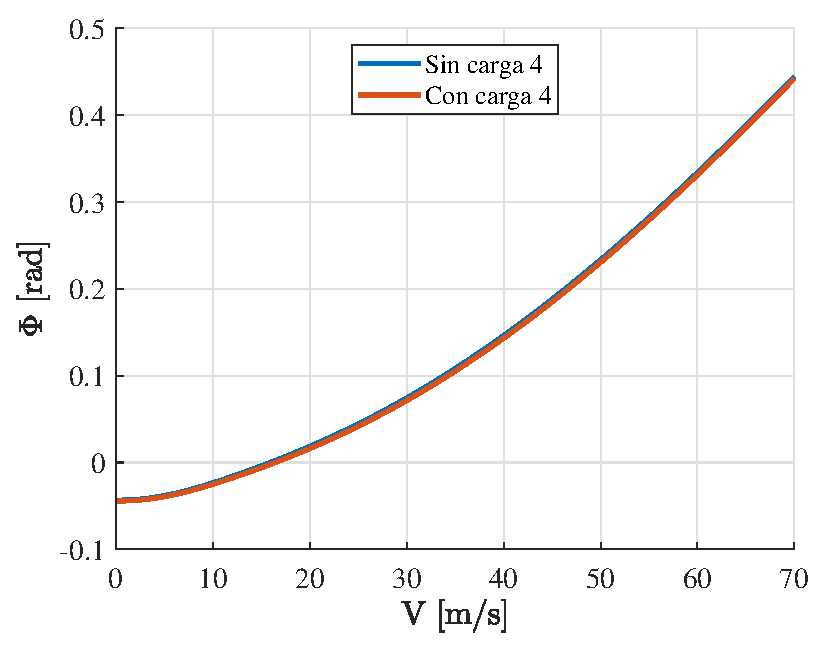
\includegraphics[width=90mm]{graficos/BalanVCSP}
	\caption{Ángulos de balanceo de la aeronave con y sin carga 4 embarcada en $l_x=0.4$ m y $l_y=-0.1$ m en función de la velocidad a 1000 m de altitud y vuelo circular de radio 300 m.}
	\label{PhiVCSP}
\end{figure}
\begin{figure}
	\centering
 	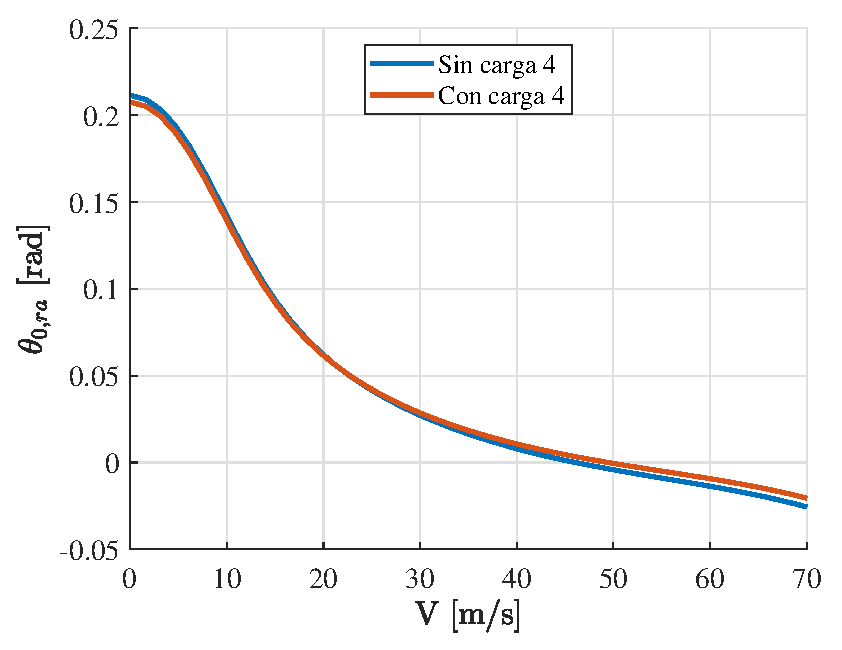
\includegraphics[width=90mm]{graficos/theta0raVCSP}
	\caption{Ángulos de paso colectivo del rotor antipar de la aeronave con y sin carga 4 embarcada en $l_x=0.4$ m y $l_y=-0.1$ m en función de la velocidad a 1000 m de altitud y vuelo circular de radio 300 m.}
	\label{Theta0raVCSP}
\end{figure}

Por último, el ángulo de paso colectivo del rotor antipar se ve suavizado con la instalación de la carga 4, disminuyendo en valor absoluto para altas y bajas velocidades hasta 0.005 rad para velocidades cercanas a los 56 m/s.


\subsubsection*{Efectos de la Posición de la Carga}

Ahora se comprobará como evolucionan los parámetros de vuelo con la posición de la carga 4 embarcada.

\begin{figure}
	\centering
	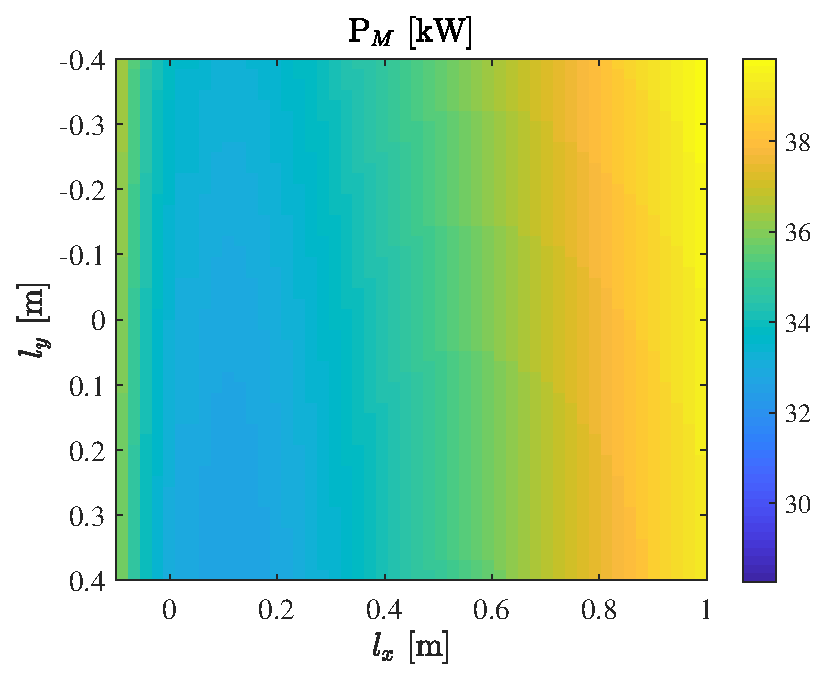
\includegraphics[width=90mm]{graficos/PMSP}
	\caption{Consumo de Potencia de la aeronave en función de la posición de la carga 4 respecto a $O_f$ para las condiciones de vuelo descritas para la embarcación de esta carga.}
	\label{PMSP}
\end{figure}

Los resultados de potencias necesarias para el vuelo se recogen en la gráfica \ref{PMSP}. En ella se pueden apreciar variaciones de hasta 7 kW en la potencia consumida por el motor en función de la posición longitudinal de la carga 4. Los valores mínimos de potencia se obtienen para la carga situada en $l_x=0.11$ m. La posición lateral, en cambio, interfiere en menor medida en el consumo de potencia, siendo ligeramente más favorable colocar la carga en el lado derecho del fuselaje.

\begin{figure}
	\centering
	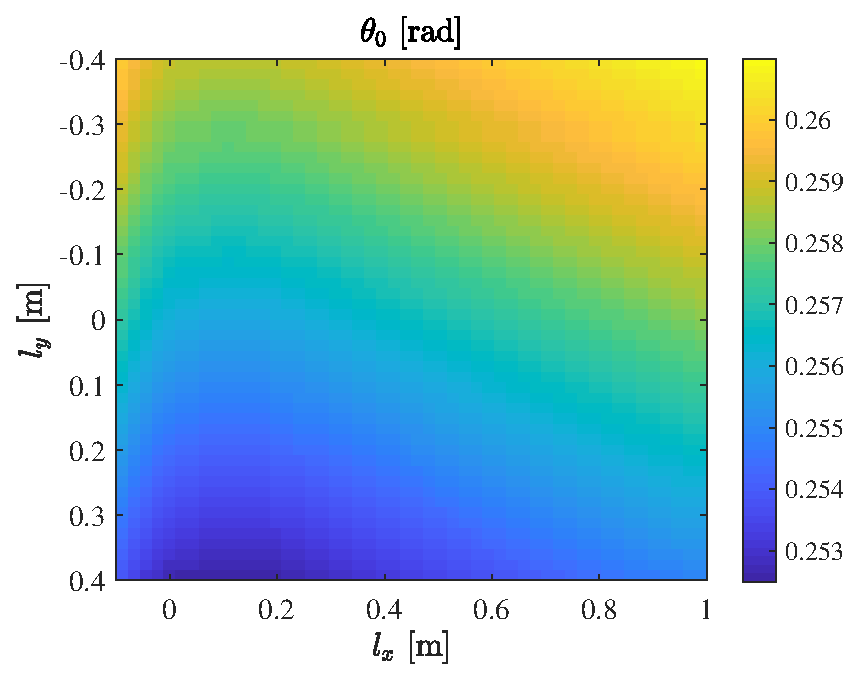
\includegraphics[width=90mm]{graficos/theta0SP}
	\caption{Ángulo de paso colectivo del rotor principal  en función de la posición de la carga 4 respecto a $O_f$ para las condiciones de vuelo descritas para la embarcación de esta carga.}
	\label{theta0SP}
\end{figure}

Las variaciones en los valores del ángulo de paso colectivo del rotor principal con la posición de la carga 4 presentan unos valores máximos de 0.008 rad, lo que supone menos de medio grado de diferencia. La gráfica \ref{theta0SP} muestra que, de nuevo, los menores valores se obtienen para una posición tal que $l_x=0.11$ m y $l_y$ lo mayor posible.

\begin{figure}
	\centering
	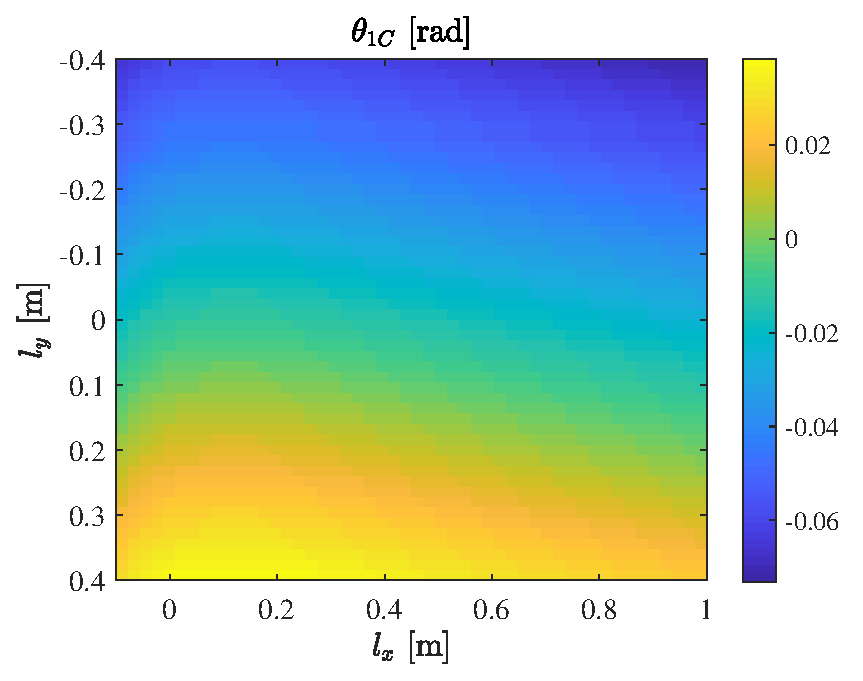
\includegraphics[width=90mm]{graficos/theta1CSP}
	\caption{Ángulo de paso cíclico longitudinal del rotor principal en función de la posición de la carga 4 respecto a $O_f$ para las condiciones de vuelo descritas para la embarcación de esta carga.}
	\label{theta1CSP}
\end{figure}
\begin{figure}
	\centering
	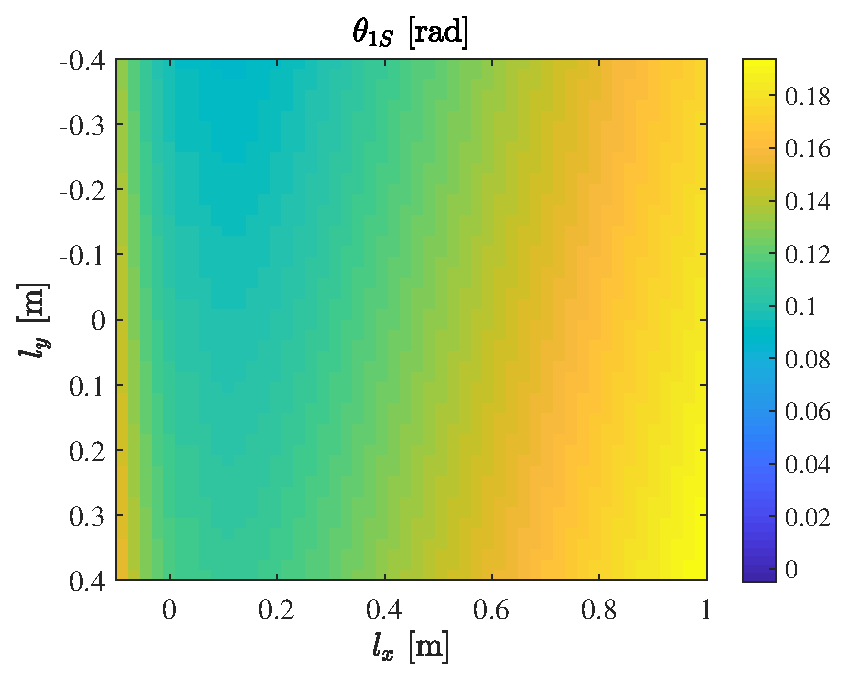
\includegraphics[width=90mm]{graficos/theta1SSP}
	\caption{Ángulo de paso cíclico lateral del rotor principal en función de la posición de la carga 4 respecto a $O_f$ para las condiciones de vuelo descritas para la embarcación de esta carga.}
	\label{theta1SSP}
\end{figure}

En lo que respecta a los pasos cíclicos, representados en las gráficas \ref{theta1CSP} y \ref{theta1SSP}, el efecto de la posición de la carga provoca cambios mayores de su valor, llegando a variaciones máximos de 0.12 rad para el paso cíclico longitudinal y 0.08 rad para el lateral.
La posición longitudinal de la carga 4 no provoca grandes variaciones en el paso longitudinal, obteniéndose aún así unos valores máximos para $l_x=0.11$ m, por lo que será mucho más importante la posición lateral, que permite alcanzar valores nulos del paso cíclico longitudinal en el intervalo de valores $l_y$ de 0 a 0.2 m, reduciéndose el ángulo con el desplazamiento hacia la izquierda de la carga.
Para el paso cíclico lateral el comportamiento se invierte, siendo el parámetro más relevante en su valor la posición longitudinal de la carga. Sus valores mínimos se alcanzan para posiciones en $l_x=0.11$ m y lo mas desplazadas posibles hacia la izquierda.

\begin{figure}
	\centering
	\includegraphics[width=90mm]{graficos/CabSP}
	\caption{Ángulo de cabeceo de la aeronave en función de la posición de la carga 4 respecto a $O_f$ para las condiciones de vuelo descritas para la embarcación de esta carga.}
	\label{CabSP}
\end{figure}

En la gráfica \ref{CabSP} se puede ver de nuevo que los efectos la posición lateral de la carga sobre el ángulo de cabeceo son despreciables. Los valores máximos de cabeceo se dan para $l_x=0.13$, siendo el valor de cabeceo negativo en todo momento en estas condiciones de vuelo. Variar $l_x$ provoca variaciones de hasta 0.08 rad en el cabeceo.

\begin{figure}
	\centering
	\includegraphics[width=90mm]{graficos/BalanSP}
	\caption{Ángulo de balanceo de la aeronave en función de la posición de la carga 4 respecto a $O_f$ para las condiciones de vuelo descritas para la embarcación de esta carga.}
	\label{BalanSP}
\end{figure}

En el caso del ángulo de balanceo tampoco hay sorpresas; la gráfica \ref{BalanSP} muestra claramente que el valor de este apenas varía con la posición longitudinal de la carga, aunque presenta un pequeño máximo para valore de $l_x$ alrededor de 0.2 m. La posición lateral por su parte si resulta muy relevante, produciendo cambios de hasta 0.1 rad entre las posibles configuraciones. Para reducir el ángulo de balanceo conviene situar la carga en la parte izquierda del fuselaje, lo que resulta obvio para trayectorias circulares con giro a derechas.

\begin{figure}
	\centering
	\includegraphics[width=90mm]{graficos/theta0raSP}
	\caption{Ángulo de paso colectivo del rotor antipar en función de la posición de la carga 4 respecto a $O_f$ para las condiciones de vuelo descritas para la embarcación de esta carga.}
	\label{theta0raSP}
\end{figure}

Por último, el ángulo de paso colectivo del rotor antipar llega a sufrir variaciones de hasta 0.012 rad. Se puede observar en la gráfica \ref{theta0raSP} que los valores mínimos de este se alcanzan para posiciones longitudinales en $l_x=0.11$ m y desplazadas lateralmente hacia la derecha, aunque el efecto de esto último es bastante menor.

Analizados los resultados, la posición más favorable sería aquella que minimizase la potencia necesaria para la operación, a la vez que reduzca en valor absoluto los diferentes ángulos de control y de Euler, permitiendo una mayor maniobrabilidad en caso de ser necesaria.
Según los datos obtenidos, esta posición será:
\begin{itemize}
	\item $l_x=0.11$ m
	\item $l_y=0.05$ m
\end{itemize}
El valor de $l_y$ no tiene que ser exactamente el expuesto, pero si debe ser pequeño positivo para optimizar los resultados.
